%----------------------------------------------------------------------------------------
%	PACKAGES AND OTHER DOCUMENT CONFIGURATIONS
%----------------------------------------------------------------------------------------

\documentclass[
11pt, % The default document font size, options: 10pt, 11pt, 12pt
%oneside, % Two side (alternating margins) for binding by default, uncomment to switch to one side
english, % ngerman for German
singlespacing, % Single line spacing, alternatives: onehalfspacing or doublespacing
%draft, % Uncomment to enable draft mode (no pictures, no links, overfull hboxes indicated)
%nolistspacing, % If the document is onehalfspacing or doublespacing, uncomment this to set spacing in lists to single
%liststotoc, % Uncomment to add the list of figures/tables/etc to the table of contents
%toctotoc, % Uncomment to add the main table of contents to the table of contents
%parskip, % Uncomment to add space between paragraphs
%nohyperref, % Uncomment to not load the hyperref package
headsepline, % Uncomment to get a line under the header
%chapterinoneline, % Uncomment to place the chapter title next to the number on one line
%consistentlayout, % Uncomment to change the layout of the declaration, abstract and acknowledgements pages to match the default layout
]{MastersDoctoralThesis} % The class file specifying the document structure

\usepackage[utf8]{inputenc} % Required for inputting international characters
\usepackage[T1]{fontenc} % Output font encoding for international characters

\usepackage{palatino} % Use the Palatino font by default

\usepackage[backend=bibtex,style=authoryear,natbib=true]{biblatex} % Use the bibtex backend with the authoryear citation style (which resembles APA)

\addbibresource{example.bib} % The filename of the bibliography

\usepackage[autostyle=true]{csquotes} % Required to generate language-dependent quotes in the bibliography

%----------------------------------------------------------------------------------------
%	MARGIN SETTINGS
%----------------------------------------------------------------------------------------

\geometry{
	paper=a4paper, % Change to letterpaper for US letter
	inner=2.5cm, % Inner margin
	outer=3.8cm, % Outer margin
	bindingoffset=.5cm, % Binding offset
	top=1.5cm, % Top margin
	bottom=1.5cm, % Bottom margin
	%showframe, % Uncomment to show how the type block is set on the page
}

%----------------------------------------------------------------------------------------
%	THESIS INFORMATION
%----------------------------------------------------------------------------------------

\thesistitle{Hand Gesture Recognition via Leap Motion Sensor} % Your thesis title, this is used in the title and abstract, print it elsewhere with \ttitle
\supervisor{Dr. Irina \textsc{Voiculescu}} % Your supervisor's name, this is used in the title page, print it elsewhere with \supname
\examiner{} % Your examiner's name, this is not currently used anywhere in the template, print it elsewhere with \examname
\degree{Masters in Computer Science} % Your degree name, this is used in the title page and abstract, print it elsewhere with \degreename
\author{Jahangir \textsc{Iqbal}} % Your name, this is used in the title page and abstract, print it elsewhere with \authorname
\addresses{} % Your address, this is not currently used anywhere in the template, print it elsewhere with \addressname

\subject{Computer Science} % Your subject area, this is not currently used anywhere in the template, print it elsewhere with \subjectname
\keywords{} % Keywords for your thesis, this is not currently used anywhere in the template, print it elsewhere with \keywordnames
\university{\href{http://www.ox.ac.uk/} {University of Oxford}} %print it elsewhere with \univname
\department{\href{http://www.cs.ox.ac.uk/} {Department of Computer Science}} % print it elsewhere with \deptname


%\group{\href{http://researchgroup.university.com} {Research Group Name}} % Your research group's name and URL, this is used in the title page, print it elsewhere with \groupname
\faculty{\href{http://faculty.university.com}{Faculty Name}} % Your faculty's name and URL, this is used in the title page and abstract, print it elsewhere with \facname

\AtBeginDocument{
\hypersetup{pdftitle=\ttitle} % Set the PDF's title to your title
\hypersetup{pdfauthor=\authorname} % Set the PDF's author to your name
\hypersetup{pdfkeywords=\keywordnames} % Set the PDF's keywords to your keywords
}

%----------------------------------------------------------------------------------------
%	MY CHANGES. START
%----------------------------------------------------------------------------------------

%------------------------------------CONFIGURATION FOR DISPLAYING CODE
\usepackage{listings}
\usepackage{color}

\definecolor{dkgreen}{rgb}{0,0.6,0}
\definecolor{gray}{rgb}{0.5,0.5,0.5}
\definecolor{mauve}{rgb}{0.58,0,0.82}

\lstset{frame=tb,
  language=Java,
  aboveskip=3mm,
  belowskip=3mm,
  showstringspaces=false,
  columns=flexible,
  basicstyle={\small\ttfamily},
  numbers=left,
  stepnumber=1,
  numberstyle=\tiny\color{gray},
  keywordstyle=\color{blue},
  commentstyle=\color{dkgreen},
  stringstyle=\color{mauve},
  breaklines=true,
  breakatwhitespace=true,
  tabsize=3
}

%------------------------------------MULTILINE COMMENTS
\usepackage{verbatim}


%------------------------------------FRAME AROUND CODE LISTING
\usepackage{listings}
\usepackage[most]{tcolorbox}
\usepackage{inconsolata}

\newtcblisting[auto counter]{codelisting}[2][]{sharp corners, 
    fonttitle=\bfseries, colframe=gray, listing only, 
    listing options={basicstyle=\ttfamily,language=java}, 
    title=Listing \thetcbcounter: #2, #1}

%------------------------------------FIGURES SIDE BY SIDE
\usepackage{lipsum}
\usepackage{mwe}%minimum working example

%------------------------------------FIGURES PLACEMENT
\usepackage{float}% If comment this, figure moves to Page 2



%----------------------------------------------------------------------------------------
%	MY CHANGES. END								START OF DOCUMENT BELOW
%----------------------------------------------------------------------------------------

\begin{document}
\frontmatter % Use roman page numbering style (i, ii, iii, iv...) for the pre-content pages
\pagestyle{plain} % Default to the plain heading style until the thesis style is called for the body content

%----------------------------------------------------------------------------------------
%	TITLE PAGE
%----------------------------------------------------------------------------------------
\begin{comment}
\begin{titlepage}
\begin{center}

\vspace*{.06\textheight}
{\scshape\LARGE \univname\par}\vspace{1.5cm} % University name

\HRule \\[0.4cm] % Horizontal line
{\huge \bfseries \ttitle\par}\vspace{0.4cm} % Thesis title
\HRule \\[1.5cm] % Horizontal line
 
\begin{minipage}[t]{0.4\textwidth}
\begin{flushleft} \large
\emph{Authors:}\\
\href{http://www.johnnysmith.com}{\authorname} % Author name - remove the \href bracket to remove the link
\end{flushleft}
\end{minipage}
\begin{minipage}[t]{0.4\textwidth}
\begin{flushright} \large
\emph{Supervisor:} \\
\href{http://www.jamessmith.com}{\supname} % Supervisor name - remove the \href bracket to remove the link  
\end{flushright}
\end{minipage}\\[3cm]
 
\vfill

\large \textit{A thesis submitted in fulfillment of the requirements\\ for the degree of \degreename}\\[0.3cm] % University requirement text
\textit{in the}\\[0.4cm]
\deptname\\[2cm] % department name
 
\vfill

{\large \today}\\[4cm] % Date
%
\includegraphics[scale=.1]{Figures/universityLogo.jpg} % University/department logo - uncomment to place it  
\vfill
\end{center}
\end{titlepage}
\end{comment}
%----------------------------------------------------------------------------------------
%	DECLARATION PAGE
%----------------------------------------------------------------------------------------
\begin{comment}
\begin{declaration}
\addchaptertocentry{\authorshipname} % Add the declaration to the table of contents
\noindent I, \authorname, declare that this thesis titled, \enquote{\ttitle} and the work presented in it are my own. I confirm that:

\begin{itemize} 
\item This work was done wholly or mainly while in candidature for a research degree at this University.
\item Where any part of this thesis has previously been submitted for a degree or any other qualification at this University or any other institution, this has been clearly stated.
\item Where I have consulted the published work of others, this is always clearly attributed.
\item Where I have quoted from the work of others, the source is always given. With the exception of such quotations, this thesis is entirely my own work.
\item I have acknowledged all main sources of help.
\item Where the thesis is based on work done by myself jointly with others, I have made clear exactly what was done by others and what I have contributed myself.\\
\end{itemize}
 
\noindent Signed:\\
\rule[0.5em]{25em}{0.5pt} % This prints a line for the signature
 
\noindent Date:\\
\rule[0.5em]{25em}{0.5pt} % This prints a line to write the date
\end{declaration}

\cleardoublepage
\end{comment}

%----------------------------------------------------------------------------------------
%	ABSTRACT PAGE
%----------------------------------------------------------------------------------------
\begin{comment}
\begin{abstract}
\addchaptertocentry{\abstractname} % Add the abstract to the table of contents
The Thesis Abstract is written here (and usually kept to just this page). The page is kept centered vertically so can expand into the blank space above the title too\ldots
\end{abstract}
\end{comment}

%----------------------------------------------------------------------------------------
%	ACKNOWLEDGEMENTS
%----------------------------------------------------------------------------------------
\begin{comment}
\begin{acknowledgements}
\addchaptertocentry{\acknowledgementname} % Add the acknowledgements to the table of contents
The acknowledgments and the people to thank go here, don't forget to include your project advisor\ldots
\end{acknowledgements}
\end{comment}

%----------------------------------------------------------------------------------------
%	LIST OF CONTENTS/FIGURES/TABLES PAGES
%----------------------------------------------------------------------------------------
\begin{comment}
\tableofcontents % Prints the main table of contents
\listoffigures % Prints the list of figures
\listoftables % Prints the list of tables
\end{comment}
%----------------------------------------------------------------------------------------
%	DEDICATION
%----------------------------------------------------------------------------------------
\begin{comment}
\dedicatory{For/Dedicated to/To my\ldots} 
\end{comment}
%----------------------------------------------------------------------------------------
%	THESIS CONTENT - CHAPTERS
%----------------------------------------------------------------------------------------
\mainmatter % Begin numeric (1,2,3...) page numbering
\pagestyle{thesis} % Return the page headers back to the "thesis" style

% Include the chapters of the thesis as separate files from the Chapters folder
% Uncomment the lines as you write the chapters
\chapter{Scoring of Gestures}

\label{Chapter5_scoring} 

\begin{comment}
-------------------------------------------------
%								Chapter layout
5. Scoring of Gestures
	a. Angle Based Comparison Function
	b. Component Based Comparison Function
-------------------------------------------------
\end{comment}

%------------------------------------------------
%	SECTION 1 Angle Based Comparison Function
%------------------------------------------------
\section{Angle Based Comparison Function}
%description of algorithm and introduction to compare() function
This is the first way by which a hand gesture is scored. This scoring method compares one hand against another; namely, it is usually comparing the user's hand versus the target hand shown on the screen that the user was trying to imitate. It uses the angles between the three foremost bones, (distal, intermediate, proximal), of the five fingers as the primary means of determining how close a user's hand is to the target hand. It also uses the angle the wrist makes to the arm in its calculations to determine the final score for the hand. Figure \ref{fig:compare1} shows some important parts of the compare() function which scores the angular similarities between two hands. This function first makes sure that the two hands that are being compared are of the same kind; ie the hands must both be left or both must be right, otherwise the result of the compare() function will be 0. It then finds angles between adjacent finger bones in both hands and compares the two angles for the amount of similarity between them. This similarity between the two angles, which is the result of the compareAngles() method call, will be a number between 0 and 1. A weight applied to this similarity measure and then the result added to the summation variable x. This function relies on some weight parameters, see Figure \ref{fig:weights}, that are set higher for the longer bones that are closer to the knuckles. For example the proximal bones have a weight of 4; the intermediate bones have a weight of 2 and the distal bones have a weight of 1. This is because the bigger bones closer to the palm of the hand are a bit more limited in their mobility. Therefore, determining correlation between these corresponding bigger bones such as proximal has a higher influence on the overall value of the compare() function. 
\begin{figure}[H]
\centering
\begin{lstlisting}
public double compare(Hand h1, Hand h2) {
	//check if both hands are of the same type.
	if (h1.isLeft() == h2.isLeft()) {
		double x = 0;
		//wrist
		x += compareAngles(angleWristArm(h1), angleWristArm(h2))* weight_wrist;
		//five fingers "proximal". compareAngles always returns between 0-1
		x += compareAngles(anglePinkyProximal(h1), anglePinkyProximal(h2))*weight_pinky_proximal;
		x += compareAngles(angleRingProximal(h1), angleRingProximal(h2))* weight_ring_proximal;
		x += compareAngles(angleMiddleProximal(h1), angleMiddleProximal(h2))* weight_middle_proximal;
		x += compareAngles(angleIndexProximal(h1), angleIndexProximal(h2))* weight_index_proximal;
		x += compareAngles(angleThumbProximal(h1), angleThumbProximal(h2))* weight_thumb_proximal;
		//five fingers "intermediate"
		x += compareAngles(anglePinkyIntermediate(h1), anglePinkyIntermediate(h2))* weight_pinky_intermediate;
		...
		//five fingers "distal"
		x += compareAngles(anglePinkyDistal(h1), anglePinkyDistal(h2))* weight_pinky_distal;
		...
		x /= totalWeight();
		return x;
	} else{
		//if comparing left hand to right hand (or vice versa), return 0
		return 0; 
	}
}
\end{lstlisting}
\caption[Angular Comparison Function]{This snippet of code shows the main skeleton of the function that determines the similarity between two hands by comparing angles between various bones in the hands.}
\label{fig:compare1}
\end{figure}


\begin{figure}[H]
\centering
\begin{lstlisting}
//weights for various bone types 
static double weight_pinky_proximal = 4;
static double weight_pinky_intermediate = 2;
static double weight_pinky_distal = 1;
...
\end{lstlisting}
\caption[Bone Weights in Angular Comparison Function]{An example of the weights set for different bone types in the pinky finger.}
\label{fig:weights}
\end{figure}


%compareAngles() function
It is also worth looking into how the compareAngles() function is defined as this function determines what percentage of the weights get applied. It takes in two angles as it parameters. These angles are determined via various functions which find angles between consecutive bones of a specific finger. An example of one such function is shown in Figure \ref{fig:angleIndexDistal} which shows how the angle between the distal bone and the intermediate bone in the index finger is determined. The angle returned by these functions will always be less than 180 degrees because of the way the angleTo() function is defined in the Leap Motion API. 
\begin{figure}[H]
\centering
\begin{lstlisting}
private float angleIndexDistal(Hand h) {
	Vector direction1 = h.fingers().get(1).bone(Bone.Type.TYPE_DISTAL).direction();
	Vector direction2 = h.fingers().get(1).bone(Bone.Type.TYPE_INTERMEDIATE).direction();
	float rawAngle = direction1.angleTo(direction2);//always less than 180
	return normalize(rawAngle, h);//flips angle on xAxis if palm facing upwards
}
\end{lstlisting}
\caption[angleIndexDistal() Function]{This function is one example of how the angles between adjacent bones are determined.}
\label{fig:angleIndexDistal}
\end{figure}

The compareAngles() is a mathematical function that determines the similarity between two angles passed into it by using the cosine trigonometry function. It will return an number between 0 and 1. It first finds the difference between the two angels. If the angles are so far apart and the distance is greater than 45 degrees, then the function will return a zero to indicate that there is not any meaningful closeness between the two angles being compared. Figure \ref{fig:compareAngles} shows this function's code. 
\begin{figure}[H]
\centering
\begin{lstlisting}
private double compareAngles(float angle1, float angle2) {
	double differenceBtwAngles = Math.abs(angle1-angle2);
	//tmp can be at most pi/4 = 45
	double tmp = Math.min(differenceBtwAngles, Math.PI/4);
	//if tmp is exactly 45, will return 0. cos(90) = 0.
	return Math.cos(2*tmp);
}
\end{lstlisting}
\caption[compareAngles() Function]{This function determines how similar (or close together) two angles using cosine.}
\label{fig:compareAngles}
\end{figure}



	


%------------------------------------------------
%	SECTION 2 Component Based Comparison Function
%------------------------------------------------
\section{Component Based Comparison Function}
The second way by which a score is assigned to a hand representing an attempted gesture will be discussed in this section. 

%descripton of algorithm
The idea behind this method is to take a given hand and decompose it into smaller component that can be scored individually. Then these components scores will be combined to arrive at the cumulative score for the entire hand. Each finger is seen as a component. After considering all of the gestures being tested in this project, I realized that each finger can be in one of three main kinds of poses. All of the fingers except for the thumb are only seen in some variations of being straight, or being curved. The thumb, however, has its own special kind of pose, which deals with connecting to other fingers. For example in some of the gestures the thumb is touching the pinky; in some gestures it is touching the middle finger. Therefore, the third possible pose is represented by a finger name, such as "pinky" or "index" etc., and it represents the finger the thumb is touching in the gesture being analyzed. The way the algorithm is designed, it makes sense to assign this dynamic third pose to the thumb only. Figure \ref{fig:gestureComponents1} and Figure \ref{fig:gestureComponents2} shows one of the gestures used in this project, namely gesture9Left, to illustrate what is meant by the different poses different components of the hand can take. As we can see, all of the fingers are straight; the ring finger is curved; and the thumb is touching the ring finger. This "pose signature" of this gesture as it is used in code is shown in Figure \ref{fig:gesture9PoseSignature}. The pose signature for a certain gesture is the same regardless of whether left or right hand is being used. That is why the code sample shows two case statements for gesture9Left and gesture9Right. 

\begin{figure}[H]
    \centering
    \begin{minipage}{0.45\textwidth}
        \centering
        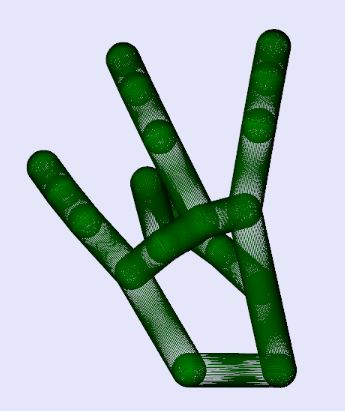
\includegraphics[scale=.5]{Figures/straight_curved_thumb1.JPG} % first figure itself
        \caption{Gesture showing different finger poses.}
		\label{fig:gestureComponents1}
    \end{minipage}\hfill
    \begin{minipage}{0.45\textwidth}
        \centering
        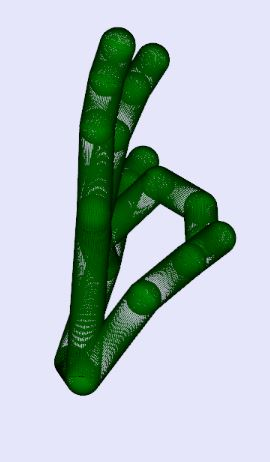
\includegraphics[scale=.5]{Figures/straight_curved_thumb2.JPG} % second figure itself
        \caption{Same gesture after a 90 degree rotation.}
        \label{fig:gestureComponents2}
    \end{minipage}
\end{figure}


\begin{figure}[H]
\centering
\begin{lstlisting}
case "gesture9Left":
case "gesture9Right":
	fingerPoseMap.put("index", "straight");
	fingerPoseMap.put("middle", "straight");
	fingerPoseMap.put("ring", "curved");
	fingerPoseMap.put("pinky", "straight");
	fingerPoseMap.put("thumb", "ring");
	break;
\end{lstlisting}
\caption[Finger Pose Mapping]{In the component based scroing, each gesture type gets a certain mapping for the kinds of poses fingers are expected to be in for that gesture.}
\label{fig:gesture9PoseSignature}
\end{figure}


% compare function and its helper functions
The comparison function for the component based scoring of hand gestures is shown in Figure \ref{fig:compare2}. It returns a number 0-100 just like the angle based comparison function to indicate the score for the hand being graded. This function gets the fingers for the hand and goes through and finds the individual grades for each finger. Then it combines the into a cumulative grade by weighing the fingers equally. 
\begin{figure}[H]
\centering
\begin{lstlisting}
public static int compare(Hand h, String gestureType) {
	FingerList fingerList = h.fingers();
	//make sure you have five fingers
	if (fingerList.count() == 5) {
		//calculate grades for each finger
		HashMap<String, Double> grades = getFingersGradedMap(getFingerHashMap(fingerList), getFingerPoseMap(gestureType));
		//grade for whole hand
		double totalGrade = cumulativeGrade(grades);
		//score 0-100
		return (int) (totalGrade * 100.0);
	}
	return -1;
}
\end{lstlisting}
\caption[Component Based Comparison Function]{}
\label{fig:compare2}
\end{figure}

To give a clearer idea about how the fingers actually get graded, the gradeFinger() function is shown in Figure \ref{fig:gradeFinger}. This function relies on three helper functions which calculate the straightness and curvedness of fingers and a function which returns the score for the thumb. 
\begin{figure}[H]
\centering
\begin{lstlisting}
private static double gradeFinger(HashMap<String, Finger> fingerMap, Finger f, String pose) {
	if (pose.equals("straight")) {
		return straightnessOfFinger(f);
	} else if (pose.equals("curved")) {
		return curvednessOfFinger(f);
	}
	//thumb is not touching any finger
	else if (pose.equals("thumb")) {
		return straightnessOfFinger(f);
	}
	//thumb touching other fingers
	else {
		Finger theFingerThumbTouches = fingerMap.get(pose);
		return getThumbScore(f, theFingerThumbTouches);
	}
}
\end{lstlisting}
\caption[gradeFinger() Function]{Given a finger a certain pose, this function returns a grade (0-1) for that finger. It uses helper functions to calculate grades for a finger in one the three main kinds of poses.}
\label{fig:gradeFinger}
\end{figure}		

Two of these helper functions, the straightnessOfFinger() and curvednessOfFinger() are shown in Figure \ref{fig:straightCurvedHelperFunctions}. These functions first find the sum of the angle between consecutive bones in the finger that is being graded. For a perfectly straight finger, the sum of these angles should be around 0 degrees. However, to allow for some leniency in the grading 30 degrees are subtracted from the sum of the angles. This allows for a buffer for the user that we intuitively as humans might guage as being relatively straight. For measuring the curvedness of a finger, the sum of the angles between the bones of the fingers should be as close to 270 as possible. However, again a buffer was provided to allow for not perfectly curled fingers to still be valid enough to return a good score.Of course these parameters can be adjusted if this application was used in the real world. These were what I felt were good parameters when I wrote these grading functions.
\begin{figure}[H]
\centering
\begin{lstlisting}
private static double straightnessOfFinger(Finger f) {
	//best case = 0; worst case is: 90+90+90 = 270.
	double sumOfAngles = getSumOfThreeAnglesBetweenFingerBones(f);
	sumOfAngles = sumOfAngles - 30;//offset by 30 degrees
	double score = sumOfAngles / 270;//closer to 0 means a better score
	score = 1 - score;//conventional scale: 0 = bad, 1 = good.
	return snapScore0to1(score);
}
private static double curvednessOfFinger(Finger f) {
	//best case is: 90+90+90 = 270; adjusted bestcase = 210; worst case = 0;
	double sumOfAngles = getSumOfThreeAnglesBetweenFingerBones(f);
	double score = sumOfAngles / 210;//closer to 1 means a better score
	return snapScore0to1(score);
}
\end{lstlisting}
\caption[straightnessOfFinger() and curvednessOfFinger()]{These helper functions are similar to each other. They are used in grading the four fingers.}
\label{fig:straightCurvedHelperFunctions}
\end{figure}		

The helper function getThumbScore(), shown in Figure \ref{fig:getThumbScore} is the more complicated of the three. The way a score is calculated for a thumb is by finding the distance between the tip bone of the thumb and any of the three outermost bones on the finger the thumb is supposed to be touching. The smallest distance is chosen as the tip of the thumb might be closer to any three of the distal, intermediate or proximal bones. This is because some people rest their thumb on the tip of the distal bone, others rest on top of the distal or the intermediate. This distance is scaled down by the smallest bone length multiplied by a scaling factor. Like the other two functions, straightnessOfFinger() and curvednessOfFinger(), the score that is returned is snapped to be between 0-1. 
\begin{figure}[H]
\centering
\begin{lstlisting}
private static double getThumbScore(Finger thumb, Finger otherFinger) {
	//bones in thumb and finger
	HashMap<String, Bone> thumbMap = getHashMapOfBonesFromFinger(thumb);
	HashMap<String, Bone> fingerMap = getHashMapOfBonesFromFinger(otherFinger);
	//get center point of thumb's tip bone
	Vector thumbTip = thumbMap.get("distal").center();
	//finger bones
	Bone d = fingerMap.get("distal");
	Bone i = fingerMap.get("intermediate");
	Bone p = fingerMap.get("proximal");
	//length of bones
	float smallestBoneLength = (Math.min(Math.min(d.length(), i.length()), p.length()));
	//distances from thumb tip to finger bones
	float d1 = thumbTip.distanceTo(d.center());
	float d2 = thumbTip.distanceTo(i.center());
	float d3 = thumbTip.distanceTo(p.center());
	double minDistance = (double) (Math.min(Math.min(d1, d2), d3));
	//scale and score
	double distanceScaledByBoneLength = minDistance / (smallestBoneLength * 3);
	double score = 1 - distanceScaledByBoneLength;
	return snapScore0to1(score);
}
\end{lstlisting}
\caption[getThumbScore() Helper Function]{This function calculates the grade for the thumb that is supposed to be touching one of the four fingers. It calculates this score by distances rather than using angles.}
\label{fig:getThumbScore}
\end{figure}

%doenst need a target hand to compare against. explain why this is good. 
One final thing to note about this comparison function is that it does not rely on a target hand for the comparison. Instead it relies on set gesture poses that are expected for the different gestures to arrive at its score. Therefore, it is more stable form of comparison. If the target hands are themselves not very good examples of the gestures being displayed, the angle based comparison method's performance could be unnecessarily affected. 
 
\begin{comment}
\chapter{Introduction}

\label{Chapter1_introduction} 

\begin{comment}
-------------------------------------------------
%								Chapter layout
1. Introduction
	a. Motivation
	b. Goals 
	c. Static Hand Gestures 
-------------------------------------------------
\end{comment}
%Computer science as a field is growing rapidly and expanding into many other disciplines including health care. This project is about very 
%short one paragraph or show explanation. maybe write abstract first. 

%------------------------------------------------
%	SECTION 1 Motivation
%------------------------------------------------
\section{Motivation}
Apraxia comes from the prefix “a” meaning “without” and the  Greek root word “praxis” which means “action”. Apraxia is a neurological condition that is sometimes caused by the effects of a stroke. It is a condition in which the patient is unable to exercise motor control over some of their muscles. The muscles themselves are not paralyzed or damaged, what causes these disorders are neurological conditions. In the department of Experimental Psychology researchers are studying patients with post-stroke loss of motor skills including possible cases of apraxia. The diagnosis of such a condition involves researchers presenting their patients with different movement based tests and evaluating the ease and effectiveness with which the patients are able to complete these screenings.  
	
%------------------------------------------------
%	SECTION 2 Goals
%------------------------------------------------
\section{Goals}
%what were the goals of this project and application. 

provide a application that clinicians can use to collect hand gesture data from patients. 
this data should be able to be scored by algorithms to determine how close their attempts are.
there will be two main functions of comparison that will be developed. 
the data collected should be able to be viewed inside the application
the data should be editable from within the app.
stored and retrieved from. 
the data should be saved to csv and outside data should be able to be loaded into the app by csv(as long as hand data is there)
the application should be easy for the users. it should not require a set position of their hand or wrist. 
the gestures shown should be rotateable. to allow from viewing from different angles. 



%------------------------------------------------
%	SECTION 3 Static Hand Gestures 
%------------------------------------------------
\section{Static Hand Gestures}
The gestures this project will be concerned with are ten gestures for the left hand and ten gestures for the right hand. These specific gestures were provided by clinicians during the first meeting with them to discuss the scope of the project. Below are some pictures showing what the target gestures that the users will have to imitate will look like in application. The gestures shown are are the ten gestures for the left hand, along with a rotated version of the same gestures to provide a different perspective into the shape of the gesture. The right hand gestures will be mirror images of the ones shown below. 
%Gesture1Left
\begin{figure}[H]
    \centering
    \begin{minipage}{0.5\textwidth}
        \centering
        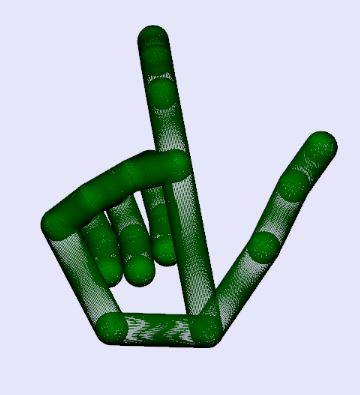
\includegraphics[scale=.75]{Figures/gesture1Left.JPG} 
        \caption[Gesture1Left]{Gesture1Left}
		\label{fig:Gesture1Left}
    \end{minipage}\hfill
    \begin{minipage}{0.5\textwidth}
        \centering
        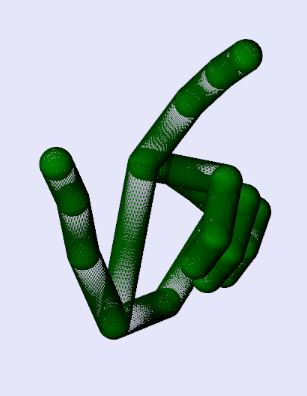
\includegraphics[scale=.7]{Figures/gesture1Left_rotated.JPG}
        \caption[Gesture1Left Rotated]{Gesture1Left rotated.}
        \label{fig:Gesture1Left_rotated}
    \end{minipage}
\end{figure}

%Gesture2Left
\begin{figure}[H]
    \centering
    \begin{minipage}{0.5\textwidth}
        \centering
        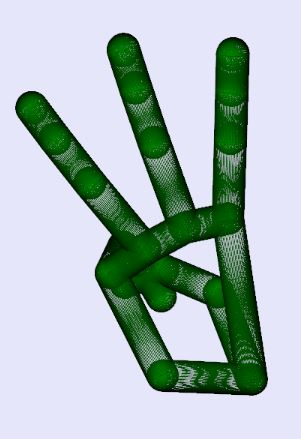
\includegraphics[scale=.75]{Figures/gesture2Left.JPG} 
        \caption[Gesture2Left]{Gesture2Left}
		\label{fig:Gesture2Left}
    \end{minipage}\hfill
    \begin{minipage}{0.5\textwidth}
        \centering
        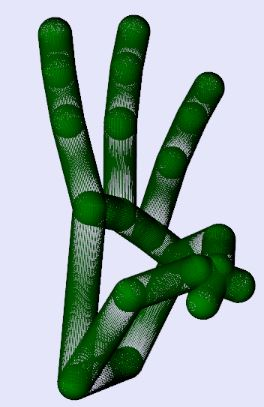
\includegraphics[scale=.75]{Figures/gesture2Left_rotated.JPG}
        \caption[Gesture2Left Rotated]{Gesture2Left rotated.}
        \label{fig:Gesture2Left_rotated}
    \end{minipage}
\end{figure}

%Gesture3Left
\begin{figure}[H]
    \centering
    \begin{minipage}{0.5\textwidth}
        \centering
        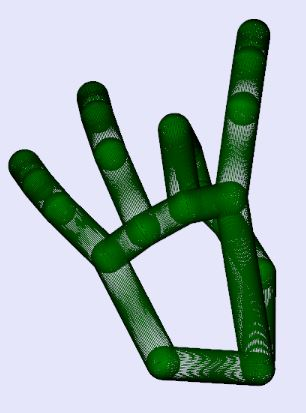
\includegraphics[scale=.75]{Figures/gesture3Left.JPG} 
        \caption[Gesture3Left]{Gesture3Left}
		\label{fig:Gesture3Left}
    \end{minipage}\hfill
    \begin{minipage}{0.5\textwidth}
        \centering
        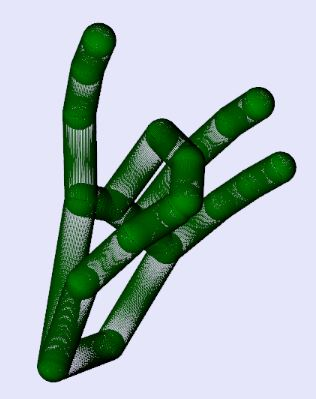
\includegraphics[scale=.75]{Figures/gesture3Left_rotated.JPG}
        \caption[Gesture3Left Rotated]{Gesture3Left rotated.}
        \label{fig:Gesture3Left_rotated}
    \end{minipage}
\end{figure}

%Gesture4Left
\begin{figure}[H]
    \centering
    \begin{minipage}{0.5\textwidth}
        \centering
        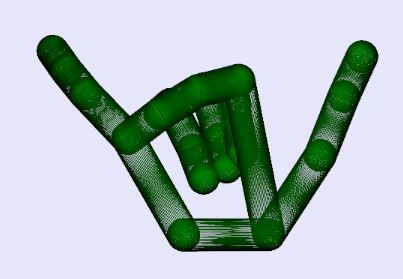
\includegraphics[scale=.75]{Figures/gesture4Left.JPG} 
        \caption[Gesture4Left]{Gesture4Left}
		\label{fig:Gesture4Left}
    \end{minipage}\hfill
    \begin{minipage}{0.5\textwidth}
        \centering
        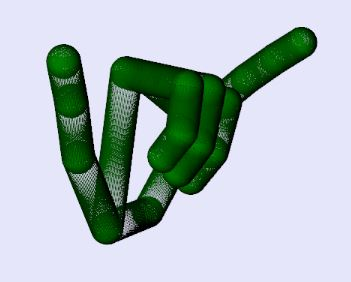
\includegraphics[scale=.75]{Figures/gesture4Left_rotated.JPG}
        \caption[Gesture4Left Rotated]{Gesture4Left rotated.}
        \label{fig:Gesture4Left_rotated}
    \end{minipage}
\end{figure}

%Gesture5Left
\begin{figure}[H]
    \centering
    \begin{minipage}{0.5\textwidth}
        \centering
        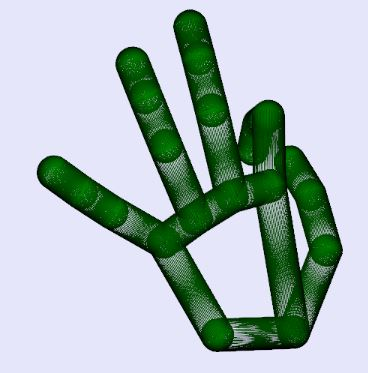
\includegraphics[scale=.75]{Figures/gesture5Left.JPG} 
        \caption[Gesture5Left]{Gesture5Left}
		\label{fig:Gesture5Left}
    \end{minipage}\hfill
    \begin{minipage}{0.5\textwidth}
        \centering
        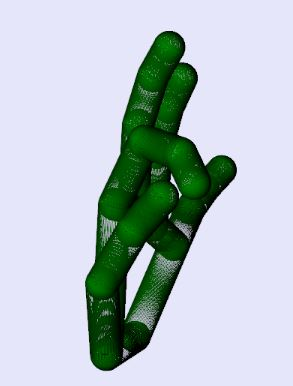
\includegraphics[scale=.75]{Figures/gesture5Left_rotated.JPG}
        \caption[Gesture5Left Rotated]{Gesture5Left rotated.}
        \label{fig:Gesture5Left_rotated}
    \end{minipage}
\end{figure}

%Gesture6Left
\begin{figure}[H]
    \centering
    \begin{minipage}{0.5\textwidth}
        \centering
        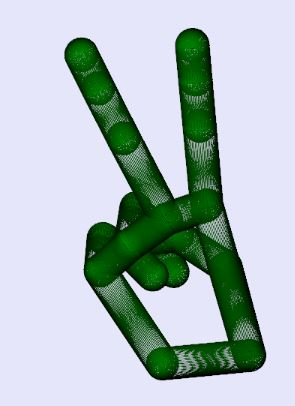
\includegraphics[scale=.75]{Figures/gesture6Left.JPG} 
        \caption[Gesture6Left]{Gesture6Left}
		\label{fig:Gesture6Left}
    \end{minipage}\hfill
    \begin{minipage}{0.5\textwidth}
        \centering
        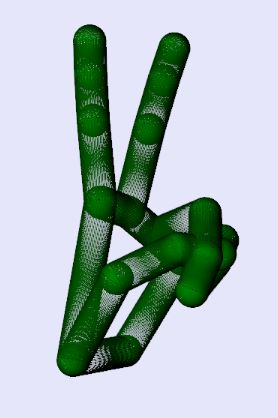
\includegraphics[scale=.7]{Figures/gesture6Left_rotated.JPG}
        \caption[Gesture6Left Rotated]{Gesture6Left rotated.}
        \label{fig:Gesture6Left_rotated}
    \end{minipage}
\end{figure}

%Gesture7Left
\begin{figure}[H]
    \centering
    \begin{minipage}{0.5\textwidth}
        \centering
        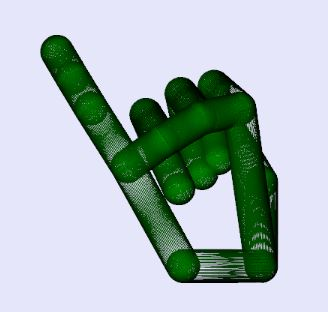
\includegraphics[scale=.75]{Figures/gesture7Left.JPG} 
        \caption[Gesture7Left]{Gesture7Left}
		\label{fig:Gesture7Left}
    \end{minipage}\hfill
    \begin{minipage}{0.5\textwidth}
        \centering
        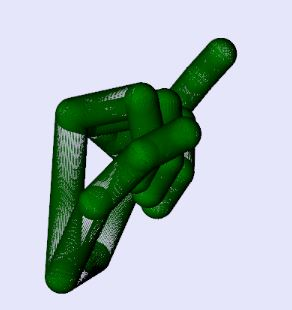
\includegraphics[scale=.75]{Figures/gesture7Left_rotated.JPG}
        \caption[Gesture7Left Rotated]{Gesture7Left rotated.}
        \label{fig:Gesture7Left_rotated}
    \end{minipage}
\end{figure}

%Gesture8Left
\begin{figure}[H]
    \centering
    \begin{minipage}{0.5\textwidth}
        \centering
        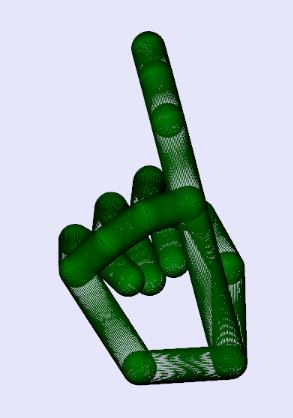
\includegraphics[scale=.75]{Figures/gesture8Left.JPG} 
        \caption[Gesture8Left]{Gesture8Left}
		\label{fig:Gesture8Left}
    \end{minipage}\hfill
    \begin{minipage}{0.5\textwidth}
        \centering
        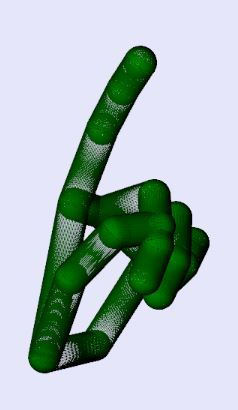
\includegraphics[scale=.75]{Figures/gesture8Left_rotated.JPG}
        \caption[Gesture8Left Rotated]{Gesture8Left rotated.}
        \label{fig:Gesture8Left_rotated}
    \end{minipage}
\end{figure}

%Gesture9Left
\begin{figure}[H]
    \centering
    \begin{minipage}{0.5\textwidth}
        \centering
        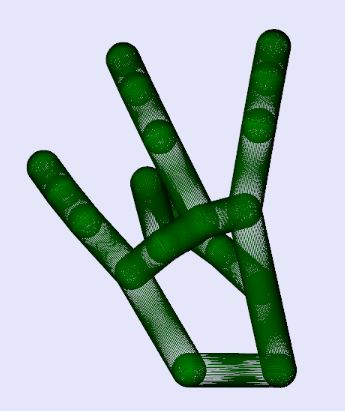
\includegraphics[scale=.75]{Figures/gesture9Left.JPG} 
        \caption[Gesture9Left]{Gesture9Left}
		\label{fig:Gesture9Left}
    \end{minipage}\hfill
    \begin{minipage}{0.5\textwidth}
        \centering
        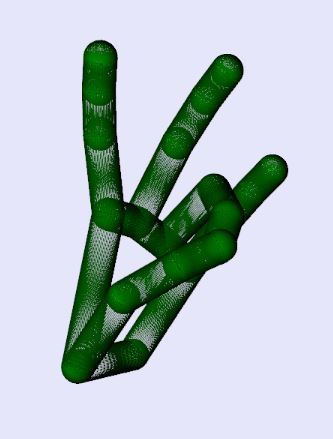
\includegraphics[scale=.75]{Figures/gesture9Left_rotated.JPG}
        \caption[Gesture9Left Rotated]{Gesture9Left rotated.}
        \label{fig:Gesture9Left_rotated}
    \end{minipage}
\end{figure}

%Gesture10Left
\begin{figure}[H]
    \centering
    \begin{minipage}{0.5\textwidth}
        \centering
        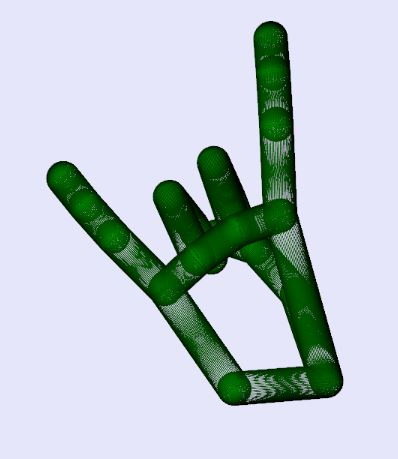
\includegraphics[scale=.75]{Figures/gesture10Left.JPG} 
        \caption[Gesture10Left]{Gesture10Left}
		\label{fig:Gesture10Left}
    \end{minipage}\hfill
    \begin{minipage}{0.5\textwidth}
        \centering
        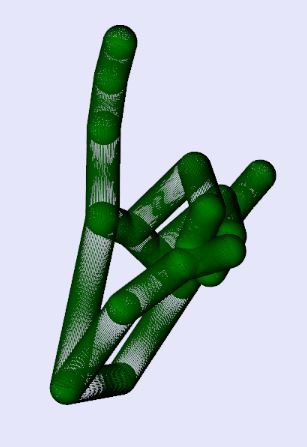
\includegraphics[scale=.75]{Figures/gesture10Left_rotated.JPG}
        \caption[Gesture10Left Rotated]{Gesture10Left rotated.}
        \label{fig:Gesture10Left_rotated}
    \end{minipage}
\end{figure}

\chapter{Background}

\label{Chapter2_background} 

\begin{comment}
-------------------------------------------------
%								Chapter layout
2. Background
	a. Leap Motion (v2)
		i. Java API and Native Libraries
		ii. Limitations of Sensor and Documentation
	b. JavaFx
		i. Java vs FXML
		ii. SceneBuilder
		iii. Jfoenix
-------------------------------------------------
\end{comment}



%------------------------------------------------
%	SECTION 1 Leap Motion (v2)
%------------------------------------------------
\section{Leap Motion}
Leap Motion controller, developed by Leap Motion Inc, US based company located in San Francisco, is a small infrared-enabled sensor that can be attached to one’s computer via a USB cable. It comes with its own software that allows it to detect a user’s hand movements in 3D space without any physical touch. It also can detect simple tools being held in the hand such as a pencil. The Leap Motion controller accomplishes this via two cameras and three embedded infrared LEDs which are able to track infrared light with wavelength outside that of the visible light spectrum. The sensor is able to detect motion in a wide space of around 8 cubic feet of area around it. This interaction area can be visualized as an inverted pyramid emanating from the Leap Motion sensor with a height, width and length of 2 cubic feet; as shown in Figure \ref{fig:LeapInteractionArea}.
\begin{figure}[th]
\centering
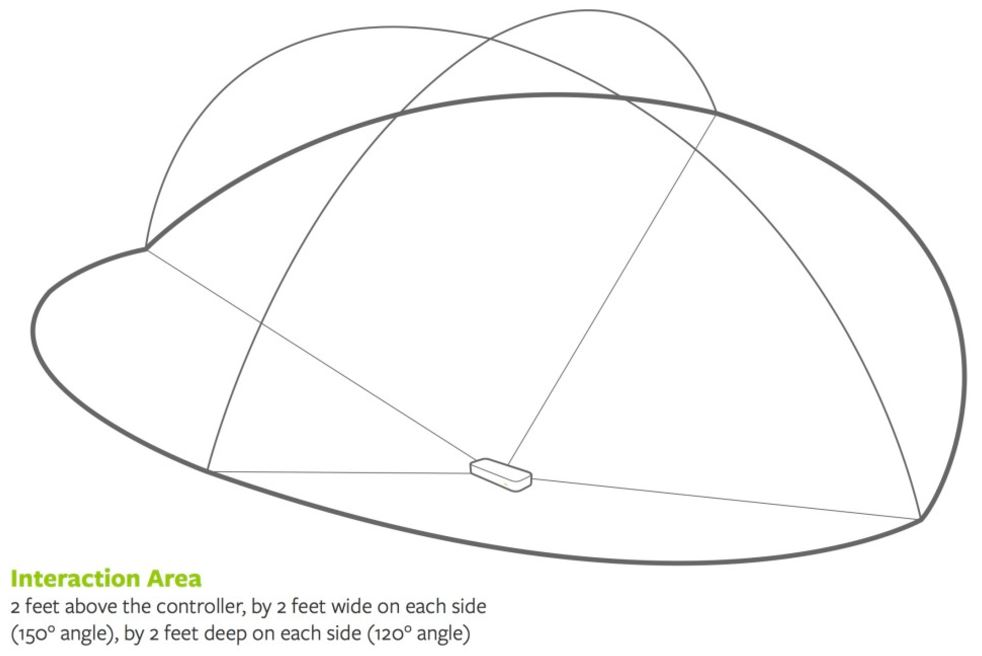
\includegraphics[scale=0.35]{Figures/LeapInteractionArea.JPG}
\caption[Leap Motion interaction area]{The area of user interaction for the Leap Motion Device.}
\label{fig:LeapInteractionArea}
\end{figure}

	
%----------------------------------- Leap Motion Java API
\subsection{Leap SDK v2 Java API}
%discuss about lm native libraries. 
When the Leap Motion software is installed on one's computer, it does not include the libraries needed in order to develop applications utilizing the controller. In order to do that, the appropriate SDK version of the software must be downloaded from Leap Motion's website. The Java SDK version includes a JAR file and two native library files. The JAR file contains the Leap Motion API class definitions and the native libraries are OS platform specific files which allow a program using the Leap Motion API to communicate to the underlying service (Windows) or daemon (Linux or Mac) which is running the Leap Controller. Setting up a Java project requires that the distributed JAR file be set to the project's classpath. When running such a project, the JVM's library path parameter must be set to the location of the native libraries.


%api/data model general discussion
In this paragraph the data model that Leap Motion uses to represent the raw data received from device's cameras will be discussed. This data model consists of Frame objects that are continuously taken at a set rate of 60fps. These Frame objects contain all of the tracked data the Leap Motion sensor recorded in its field of view at a certain instance in time. The objects that the device keeps track include the two hands, their fingers and arm positions as estimated by normal human proportions. There are corresponding Java classes to represent these objects, such as the Hand, Finger, and Arm class. There is also a Bone class to represent specific types of bones in a hand. The Leap Motion Hand model is able to provide information about the identity, position, direction, rotation angles and other characteristics of the detected hand that it represents. This Hand model also contains methods which allow one to access other model objects contained within it; for example the fingers or the arm. Leap Motion software uses an internal hand model of the human hand to assist it in making predictions about the positions of certain parts of the hand even if they are not visible to the infrared cameras and thus not able to be calculated from the tracking data. The API also provides a Vector class that allows for useful math operations involving vectors such as finding the distance, dot product or cross product between them. 

%specific example
To understand the Leap Motion Java API more clearly, a very simple example will be presented that shows how the Frame data can be received from the device. Firstly, it is assumed that the project has been set up with the correct classpath for the Leap Motion Java SDK JAR file and run time parameters pointing to the appropriate native libraries. Figure \ref{fig:leapMotionSample} shows the basic set-up required to receive data from the controller using the Leap Java API. 

\begin{figure}[th]
\centering
\begin{lstlisting}
import com.leapmotion.leap.*;

//Listener class which handles various events for the Controller
class SampleListener extends Listener {
    //method to handle the event of a Frame received from Controller
    public void onFrame(Controller controller) {
        // Get the most recent frame and report some basic information
        Frame frame = controller.frame();
        System.out.println("Frame id: " + frame.id() + ", hands: " + frame.hands().count()
    }
}

class Sample {
    public static void main(String[] args) {
        // Create leap motion controller instance
        Controller controller = new Controller();

        // Have the sample listener receive events from the controller
        controller.addListener(new SampleListener(););

        // Remove the sample listener when done
        controller.removeListener(listener);
    }
}
\end{lstlisting}
\caption[Leap Motion Sample]{This code sample shows how to connect to and receive data from the Leap Motion controller device.}
\label{fig:leapMotionSample}
\end{figure}





%------------------------------------------------
%	SECTION 2 JavaFX
%------------------------------------------------
\section{JavaFx}
JavaFX is a framework provided by Oracle Corporation that is intended to replace the Swing framework as the standard GUI library for developing desktop applications that can be run on any platform that supports Java. Since the JavaFX 2.0 release, JavaFX application can be written in pure Java code. Before that release, applications written using JavaFX libraries had to be written in JavaFX Script, a scripting language designed and used specifically for the purpose of creating GUI applications with JavaFX. This project uses the latest version of this framework, JavaFX 8, which also added support for 3D graphics and sensor support. 


%----------------------------------- Java vs FXML
\subsection{Java vs FXML}
When writing a JavaFX application, there are two very different approaches that can be used to create the actual user interface (UI) for the application. These are pure Java code and FXML. A brief introduction both of these approaches will be given below. 

The pure Java approach constructs the JavaFX application scene graph procedurally through code. Below is a simple “Hello World” program that shows a quick example of this approach in action.
\begin{figure}[th]
\centering
\begin{lstlisting}
public class HelloWorld extends Application {
public static void main(String[] args) {
	launch(args);
}

@Override
public void start(Stage primaryStage) {
	primaryStage.setTitle("Hello World!");
	Button btn = new Button();
	btn.setText("Say 'Hello World'");
	btn.setOnAction(new EventHandler<ActionEvent>() {
		@Override
		public void handle(ActionEvent event) {
			System.out.println("Hello World!");
		}
	});
	
	StackPane root = new StackPane();
	root.getChildren().add(btn);
	primaryStage.setScene(new Scene(root, 300, 250));
	primaryStage.show();
}
}
\end{lstlisting}
\caption[JavaFX HelloWorld]{A simple hello world program using JavaFX written using just Java code.}
\label{fig:helloWorldJavaFX1}
\end{figure}
This small snippet of code contains the overall structure and all of the basic components of a JavaFX application. The first point to note is that the main class which will run the JavaFX application must extend from the abstract base class called javafx.application.Application and implement is abstract start() method. The start() method serves as the main entry point for all JavaFX applications. In the application’s main() method, which is common to all Java applications, a call must be made to the launch() method which is a method defined in the base Application JavaFX class that actually launches the application in doing so makes a call to the start() method. 

The start() method receives a parameter of type Stage which serves as the primary Stage object for the application. Stage is the top-level user interface container object used by JavaFX to house the whole application. In colloquial terms it can be considered to be the “window” object of the whole application. The Stage object is has a setScene() method which requires a Scene object to be passed in. Scene class is the container of current content being displayed by the application. An application can have multiple scenes which display different pages of the the application. In JavaFX, the actual UI components, such as the StackPane layout Node shown in the simple HelloWorld example above, must be added to the Scene object in order for them to be displayed. This relationship between the Stage, Scene and “root” Node components of a JavaFX application is depicted in Figure \ref{fig:stageSceneRoot}.
\begin{figure}[th]
\centering
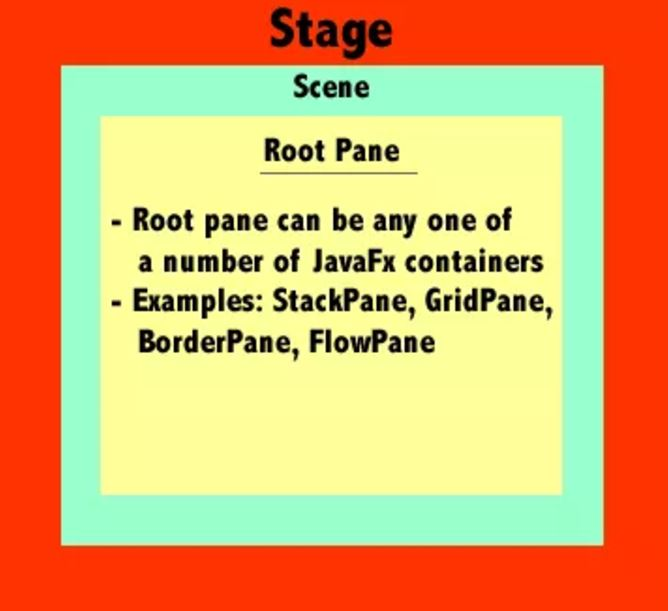
\includegraphics[scale=0.5]{Figures/stageSceneRoot.JPG}
\caption[UI Layout]{The layout components of every JavaFX application.}
\label{fig:stageSceneRoot}
\end{figure}

The UI components all extend from a parent Node class. One of the improvements that JavaFX brought in regards to its predecessor Swing, is that it represents the entire content of the scene as a tree. More specifically, all of the nodes displayed in a Scene container object must extend from a root level node and be part of the hierarchical scene graph of nodes. Figure \ref{fig:javafxSceneGraph}  displays an example of the JavaFX scene graph.
\begin{figure}[th]
\centering
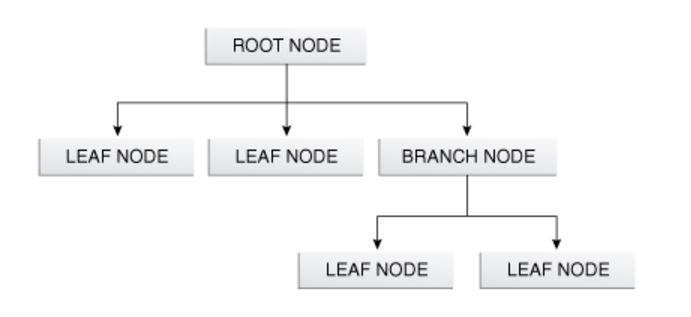
\includegraphics[scale=0.5]{Figures/javafx_scenegraph.JPG}
\caption[JavaFX Scene Graph]{The Scene Graph architectural model for UI components in JavaFX applications.}
\label{fig:javafxSceneGraph}
\end{figure}

Now that the pure Java code approach of writing JavaFX applications has been introduced, let us discuss the other approach to writing JavaFX applications; FXML. FXML is an XML-based language created by Oracle Corporation for the purpose of making it easier to define the UI of a JavaFX application. While the pure Java code approach is a much more imperative and procedural way to write JavaFX applications, FXML is a more declarative way. It resembles HTML and can also reference a controller Java class which can access and modify the UI elements defined in the FXML file. Figure \ref{fig:simpleFXML} shows a very simple FXML file that creates a VBox layout and adds a button to it. This FXML file also has a Java controller class attached to it which is called MyController.java and shown in Figure \ref{fig:simpleController}

\begin{figure}[th]
\centering
\begin{lstlisting}
<?xml version="1.0" encoding="UTF-8"?>
<?language JavaScript?>
<?import javafx.scene.control.*?>
<?import javafx.scene.layout.*?>

<VBox fx:id="myView" layoutX="10.0" layoutY="10.0" xmlns:fx="http://javafx.com/fxml/1" xmlns="http://javafx.com/javafx/2.2" fx:controller="MyController">
  <children>
    <Button fx:id="okBtn" alignment="CENTER_RIGHT" contentDisplay="CENTER" mnemonicParsing="false" onAction="#printHelloWorld" text="Say Hello World" textAlignment="CENTER" />
  </children>
</VBox>
\end{lstlisting}
\caption[FXML example]{A FXML file defining a simple layout and referencing a controller java class.}
\label{fig:simpleFXML}
\end{figure}


\begin{figure}[th]
\centering
\begin{lstlisting}
public class MyController {
	@FXML
	private void initialize() 
	{
	// this method runs first after all the UI components have been loaded and bound.
	}
	@FXML
	private void printHelloWorld() 
	{
		System.out.println("hello world!");
	}
}
\end{lstlisting}
\caption[Controller for FXML]{A controller for the FXML file. The "FXML" annotation in is used to bind certain elements to Java objects in the class.}
\label{fig:simpleController}
\end{figure}

The result from both of these HelloWorld examples will be as showing in Figure \ref{fig:helloWorldResult}. The large difference between these two approaches makes it difficult to combine them effectively, but it is possible to use them in conjunction with each other. This project takes such an approach. For the UI construction of the user's hand model, the pure Java code approach was taken. However, for the interface of the application the table construction showing all of the collected data, the FXML approach was taken. 

\begin{figure}[th]
\centering
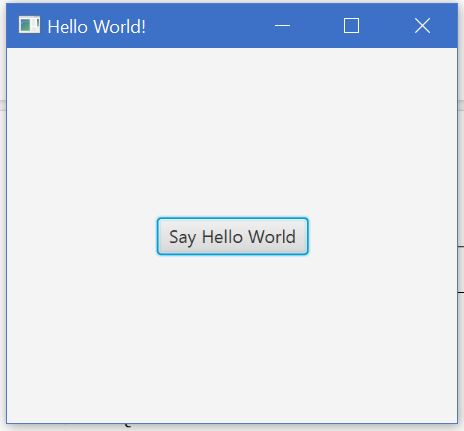
\includegraphics[scale=0.5]{Figures/helloWorldResult.JPG}
\caption[JavaFX Application Output]{The output of the simple HelloWorld application.}
\label{fig:helloWorldResult}
\end{figure}

One of the things that should be discussed is how communication can happen between different components of the application when FXML files are being used. There is a special class called FXMLLoader which is used to load FXML files and return the object graph of UI components these files contain. The FXMLLoader contains two \verb {load()} methods one of which is a static class method and the other is an instance method. The important difference between these two methods is that that instance \verb {load()} method can be used to gain access to the controller for the FXML class being loaded. Gaining access to the controller object for an FXML file in other other parts of an application is very important if one has to pass parameters into the view to change the interface. Figure \ref{fig:fxmlLoaderCode} this key difference between the two methods. 


\begin{figure}[th]
\centering
\begin{lstlisting}
// The approach uses the static "load" method. Not recommended
Parent root = FXMLLoader.load(getClass().getResource("fxml_example.fxml"));
 
//This approach allows one to access the controller. 
//create instance of FXMLLoader
FXMLLoader loader = new FXMLLoader(getClass().getResource("fxml_example.fxml"));
//get the controller
MyController controller = loader.<MyController>getController();
//initialize controller with custom parameters
controller.initData(data);
//object graph root handle
Parent root = (Parent) loader.load();
\end{lstlisting}
\caption[FXMLLoader]{Retrieving a reference to the controller object for a loaded FXML file.}
\label{fig:fxmlLoaderCode}
\end{figure}




%----------------------------------- SceneBuilder
\subsection{Scene Builder}
Scene Builder is a software that can be installed on one's computer to help design the UI and layout of a JavaFX application. It allows the user to drag and drop components from the library of available components to the central work area where they can be modified and their properties tweaked. This software is a free and open source tool that used to be developed by Oracle Corporation, but is now backed by Gluon. The easy to use drag and drop functionality of the Scene Builder allows for easy design and rapid iteration. The associated FXML code with UI created by Scene Builder can be incorporated into the JavaFX application. Using Scene Builder code bindings can also be placed on certain UI components to allow for them to execute specific logic that can be defined in the controller class of the FXML file. Figure \ref{fig:sceneBuilderWindow} shows the main layout of the Scene Builder application. There are four main panels of information that have been labeled appropriately in the figure. These are: the Library panel, which contains all of the UI components available for use; the Document panel, which shows the object graph hierarchy of the current scene being built; the Content panel, which shows the work area for user interaction; and finally the Inspector panel, which shows the various properties and layout parameters which can be modified for the currently selected UI component, as well as the various code bindings that can be placed on it. 

\begin{figure}[th]
\centering
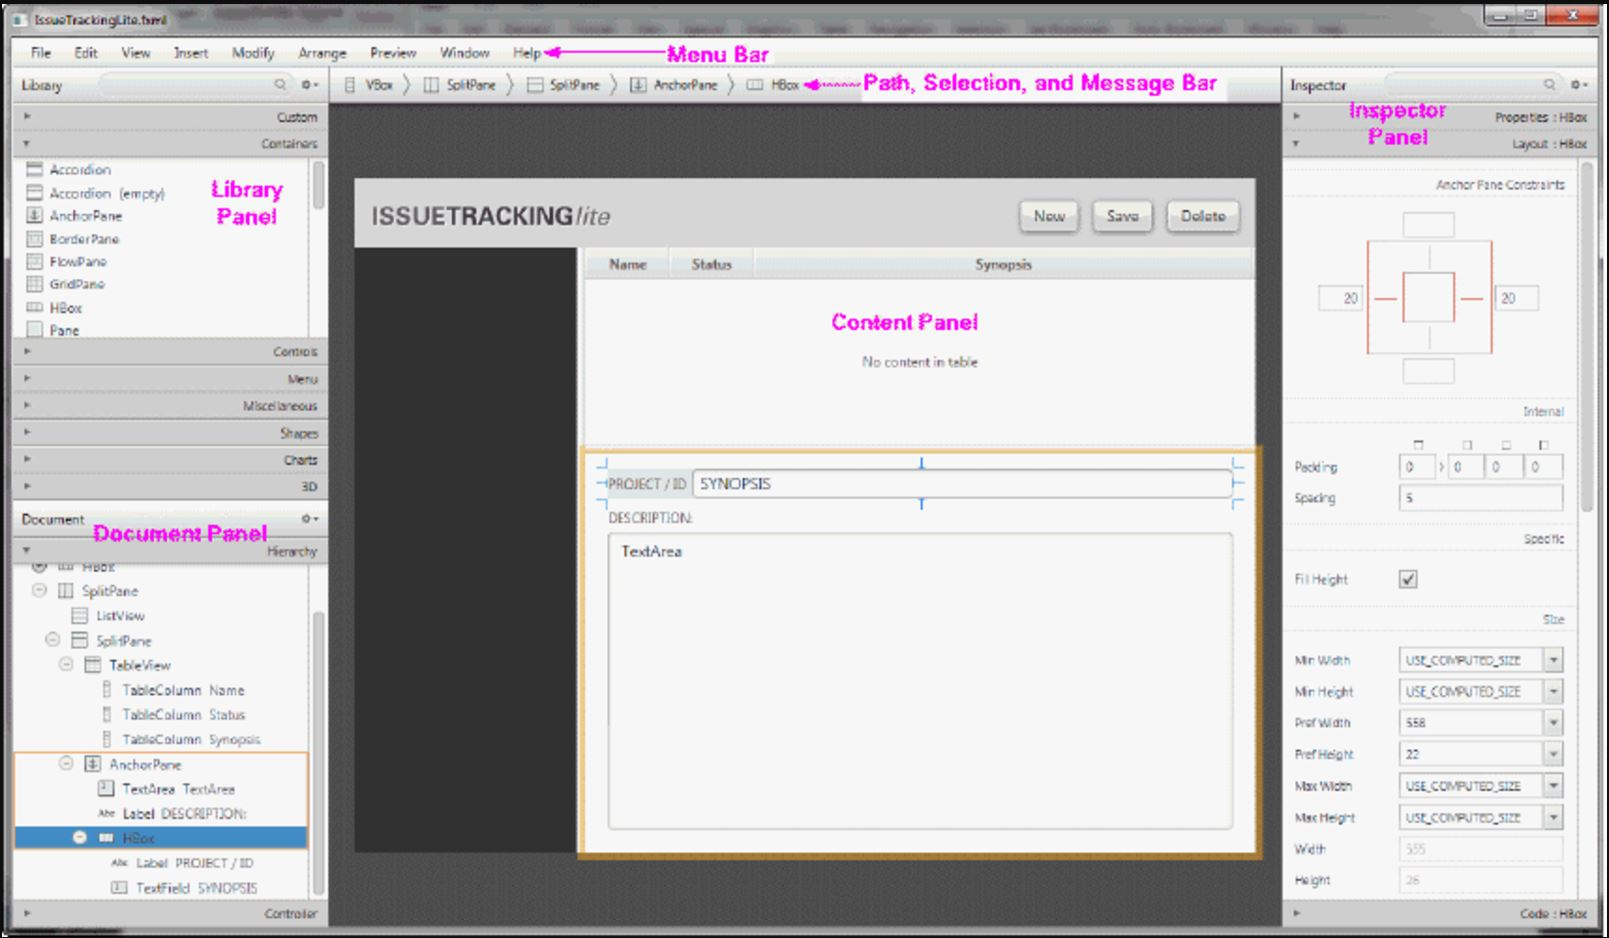
\includegraphics[scale=0.35]{Figures/sceneBuilderWindow.JPG}
\caption[Scene Builder]{This shows the different areas of interest in the Scene Builder software.}
\label{fig:sceneBuilderWindow}
\end{figure}




%----------------------------------- Jfoenix
\subsection{Jfoenix Library}
Jfoenix is a library that is used in this project. This is an open source Java library that implements Google Material Design for JavaFX components. This library can be included as a dependency via the Maven using the commands:  
\begin{lstlisting}
<dependency>
    <groupId>com.jfoenix</groupId>
    <artifactId>jfoenix</artifactId>
    <version>1.4.0</version>
</dependency>
\end{lstlisting}

Maven is a build automation tool that can also serve as a package manager that makes finding and installing dependencies simple. This library will be downloaded from Maven 2 Central Repository. To include this Jfoenix library within Scene Builder, one has to find where the JAR file for the Jfoenix library was downloaded. Then, going to Scene Builder, clicking on the gear icon in the Library panel will show a drop-down menu which has the option for "Import JAR/FXML File" as depicted in Figure \ref{fig:addLibrarySceneBuilder}. Selecting this option will allow for the Jfoenix JAR file to be specified and the custom components to be loaded into the Scene Builder. 
\begin{figure}[th]
\centering
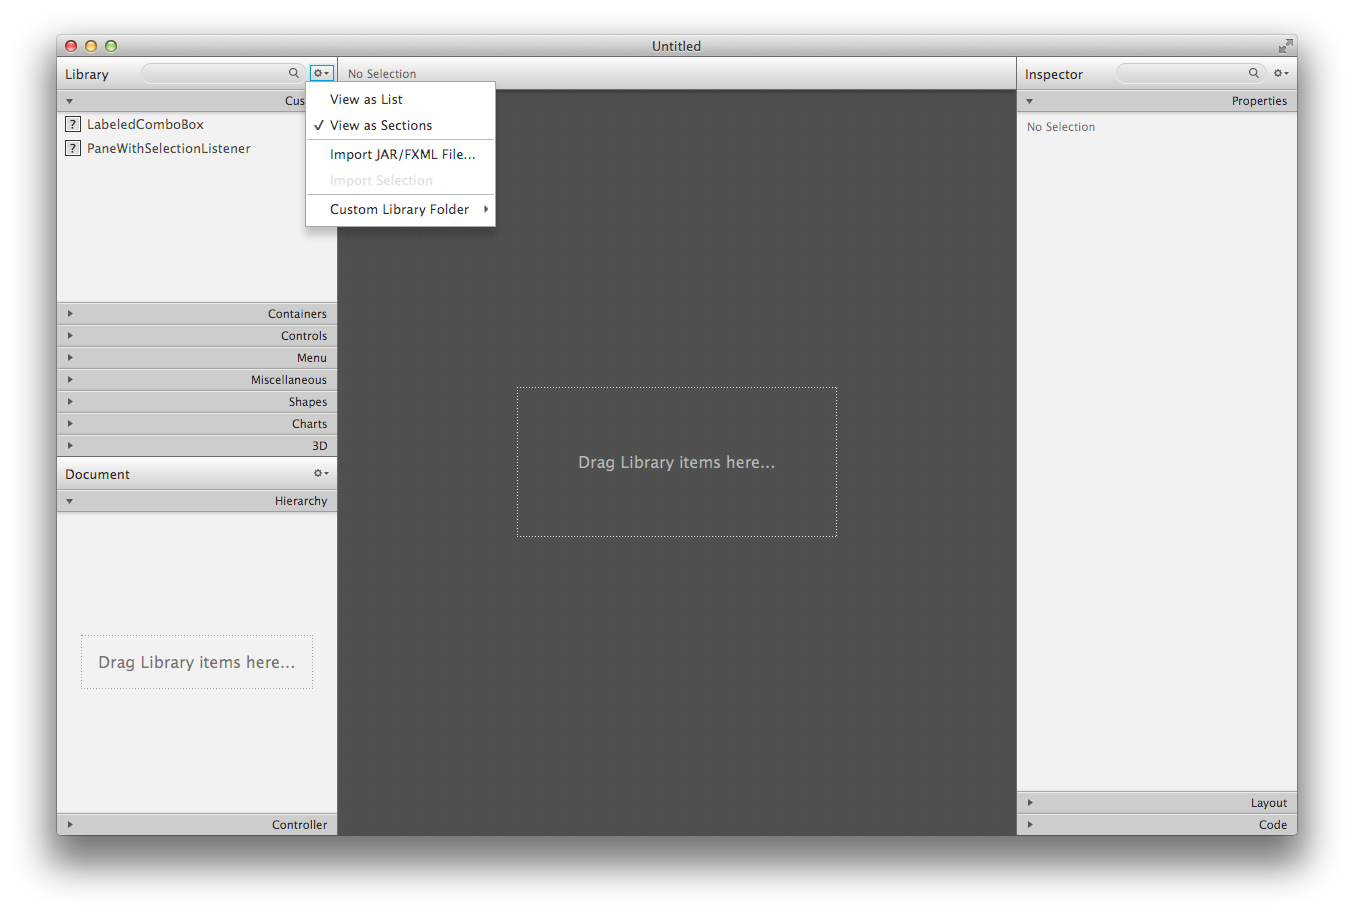
\includegraphics[scale=0.35]{Figures/addLibrarySceneBuilder.png}
\caption[External Libraries]{This is how to add a external library of custom components to the Scene Builder for UI prototyping.}
\label{fig:addLibrarySceneBuilder}
\end{figure}

\chapter{Constructing Hand UI Model}

\label{Chapter3_uiHandModel} 

\begin{comment}
-------------------------------------------------
%								Chapter layout
3. Constructing Hand UI Model
	a. Basic 3D Modelling
	b. Set Location Method
	c. Concurrency
		i. JavaFX Concurrent Package
		ii. Project Application
		
		
-------------------------------------------------
\end{comment}



%------------------------------------------------
%	SECTION 1 Basic 3D Modeling
%------------------------------------------------
\section{Basic 3D Modeling}
The Leap Motion Java API’s Hand class contains all the possible functions one might need to use when gaining more information about the hierarchical structure of this Java object. For example, given a Hand class object “hand”, we can access the fingers objects for this hand via “hand.fingers()”.  Each Finger object contains four Bone objects which are indexed from 0-3. The Bone class does contain an Enum Type that allows one to easily access them via their anatomical names (distal, intermediate, proximal, metacarpal) rather than just using a numerical index. In abstract terms, the Bone object is a vector of sorts and the ends of this bone vector represent the joints at which the bone attaches to its neighboring bones. These “joints” can be accessed via the prevJoint() and nextJoint() methods which respectively return a vector position of the Bone closer to the wrist and of the Bone object endpoint closer to the tip of the finger. The Figure \ref{fig:HandBones} shows the bones and joints of the hand for which the Leap Motion sensor records data.  

\begin{figure}[th]
\centering
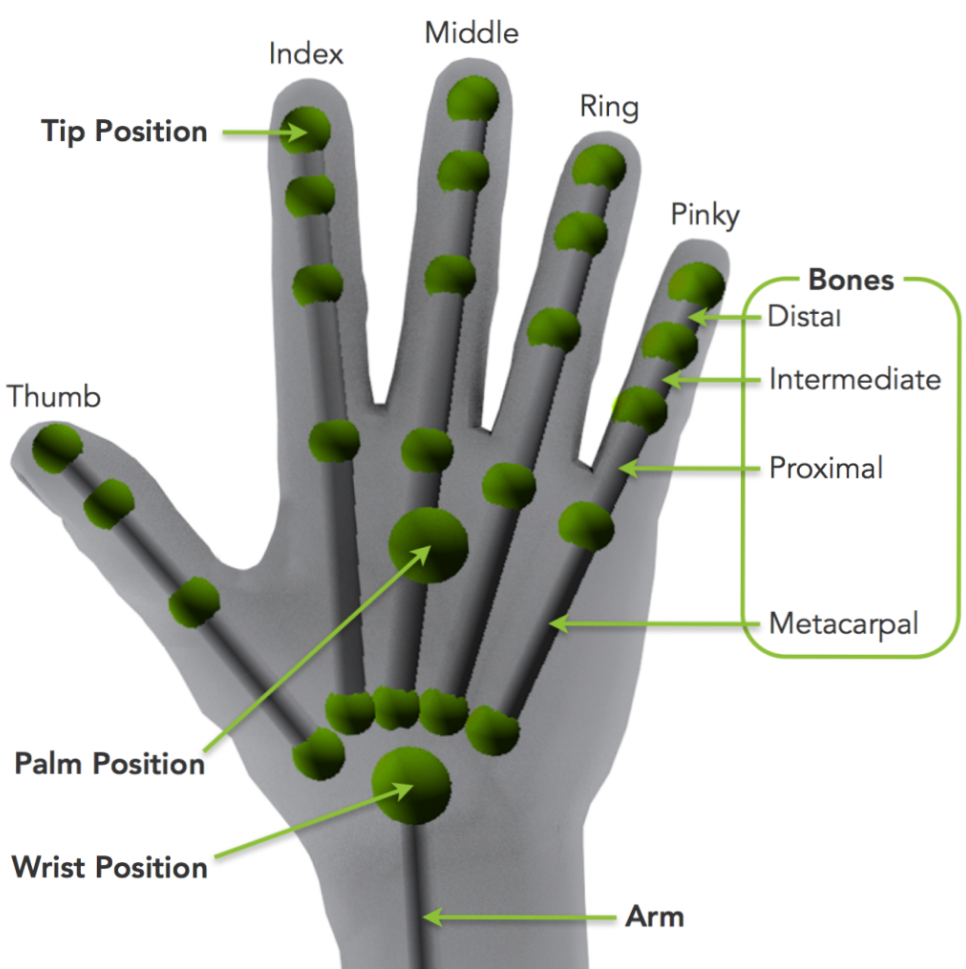
\includegraphics[scale=0.5]{Figures/handBones.png}
\caption[Hand Bone Model]{The Bones of the hand that Leap Motion device records data on. }
\label{fig:HandBones}
\end{figure}

A Hand object is only valid if it is detected by the Leap Motion device to be a physical object; if a Hand object is created via code using the Hand() constructor, that hand is considered “invalid” and will return true when the hand.invalid() method is called it. The information contained within a valid Hand object read in from the device is Read Only and can not be changed or updated. 

The Leap Motion device records numerical data about the hand and finger positions. Using the Hand class provided by the Leap Motion Java API and described above in the previous paragraph, a graphical model was constructed. For this GUI construction, a graphical representation of the hand was built using basic 3D geometric classes provided by the JavaFX framework. The bones of the hand model were represented by the Cylinder class and the joints were represented by the Sphere JavaFX class. This Hand model is contained inside the \verb UIHand_Simple Java class. This class extends a base abstract UIHand class which itself inherits from the JavaFX class called Group. Group is a type of Node in JavaFX that contains an ObservableList of children Nodes that will be added to the JavaFX Scene Graph in the order that they are added to the Group. An important point to note is that any transform, effect or property change applied to a Group will also be applied to all the children of that group. The Figure \ref{fig:javafxGroupNode} shows an example of how a Group Node can can contain multiple children nodes.

\begin{figure}[th]
\centering
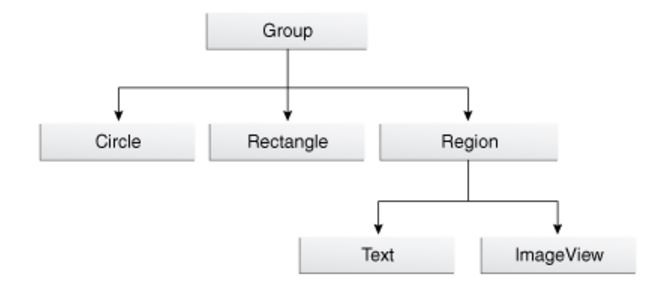
\includegraphics[scale=0.75]{Figures/javafx_group_node.JPG}
\caption[JavaFx Group Node]{The Group Node structure in the JavaFX framework. }
\label{fig:javafxGroupNode}
\end{figure}


The \verb UIHand_Simple class stores all the fingers bones in two dimensional array of Cylinder objects and all the respective joints in a different two dimensional array of Spheres. These arrays are of dimensions 5x3 to account for the five fingers and the three types of primary finger bones: distal, intermediate and proximal. In addition to these arrays, there is an array containing the four metacarpal bones of the hand; the thumb does not have a corresponding metacarpal bone like the other fingers. The also contains two more cylinders and a sphere to construct the palm section of the hand. To provide the hand with a uniform, well-blended color shading a PhongMaterial object is set as the hand’s material property. Figure \ref{fig:uihandsimpleConst} shows the initialization of the \verb UIHand_Simple and part of its constructor to illustrate how the hand model was designed.


\begin{figure}[th]
\centering
\begin{lstlisting}
public class UIHand_Simple extends UIHand {
    private static float fingerRadius = 14f;
	//Hand elements
    private Cylinder[][] fingerBones;
    private Sphere[][] fingerJoints;
    private Cylinder[] knuckleSpans;
	...
    public UIHand_Simple(Color color, boolean wireframe) {
        //Execute the Group constructor
        super();
        //Create the materials
        PhongMaterial dark = new PhongMaterial(color);
        PhongMaterial light = new PhongMaterial(color.brighter());
        //Initialize Finger bones
        fingerBones = new Cylinder[5][];
        for (int i = 0; i < 5; ++i) {
            fingerBones[i] = new Cylinder[3];
            for (int j = 0; j < 3; ++j) {
                fingerBones[i][j] = new Cylinder();
                //set material and radius and drawMode
                fingerBones[i][j].setMaterial(dark);
                fingerBones[i][j].setRadius(fingerRadius / ViewMath.radiusScaleFactor);
                if (wireframe) fingerBones[i][j].setDrawMode(DrawMode.LINE);
            }
		...
\end{lstlisting}
\caption[UIHandSimple Constructor]{A snippet of code showing how a the UIHandSimple class, representing the graphical hand, is constructed.}
\label{fig:uihandsimpleConst}
\end{figure}

Each element of the hand, such as all the cylinders and spheres representing the various bones and joints, is added to the children of the encompassing parent group that represents the hand.


%------------------------------------------------
%	SECTION 2 Set Location Method
%------------------------------------------------
\section{Set Location Method}
The \verb UIHand_Simple class also contains a method that allows for the graphical hand to be positioned according to the exact positions recorded in a Leap Motion Hand object. This method, which is called setLoc(Hand h), goes through each of the fingers and their respective bones and joints and sets the position and rotation of these these JavaFX nodes based upon the Hand object passed in. This method relies on a helper class called ViewMath which contains static methods that are called to position each individual cylinder representing a bone. Two of the important methods in ViewMath are setPositionByVector(Node n, Vector v) and setRotationByVector(Node n, Vector v). The method setPositionByVector sets the translate properties of the JavaFX Node passed in to the XYZ position recorded in the vector. The setRotationByVector method rotates the JavaFX Node passed into it by the direction which is represented by the second argument vector. This method first takes the direction and “corrects” it by flipping the z-value. This is done because JavaFX's coordinate system has the Z-axis increasing outward from the computer screen, while Leap Motion has the Z-axis increasing into the screen. The setRotationByVector finds the angle of rotation finding the the angle of the passed in direction to the Y-axis. In addition to the angle of rotation, the axis upon which the rotation will occur also needs to be defined. The axis of the rotation is found by taking the cross-product between the Y-axis and the “corrected” direction. Figure \ref{fig:setRotationByVectorCode} shows how rotation is set for nodes in the hand model.


\begin{figure}[th]
\centering
\begin{lstlisting}
//This method rotates a given JavaFx node to point in the direction passed in
public static void setRotationByVector(Node node, Vector direction) {
	//Correct the direction to correspond to JavaFx Coordinate system
	Vector correctedDirection = new Vector(direction.getX(), direction.getY(), -direction.getZ());
	//Find the angle of the direction to the y-axis; in degrees
	double angle = correctedDirection.angleTo(Vector.yAxis()) * 180 / Math.PI;
	//Find the axis of rotation by taking the cross product of the corrected direction with the y-axix
	Point3D axis = vectorToPoint(correctedDirection.cross(Vector.yAxis()));
	//Set the axis and angle of rotation on the Node object
	node.setRotate(angle);
	node.setRotationAxis(axis);
}
\end{lstlisting}
\caption[setRotationByVector Method]{A snippet of code showing how the rotation is set for an arbitrary Node object of the JavaFX Hand Model.}
\label{fig:setRotationByVectorCode}
\end{figure}




%------------------------------------------------
%	SECTION 3 Concurrency
%------------------------------------------------
\section{Concurrency}
One of the key concepts that is used in writing this project's application was that of concurrency. Concurrency in a JavaFX application is very important as it allows for the UI of to be responsive to user interactions despite the fact that the application might also be executing other tasks in the background. In other to achieve this requirement, it is necessary to employ multi-threading so that the main application thread can focus on responding to user interactions and other time-consuming tasks can be delegated to background threads. The UI in a JavaFX application is represented by the Scene Graph, which has been discussed earlier. The Scene Graph is not thread-safe and it should only be accessed and updated via the main running application thread, which is called the JavaFX Application thread. Implementing long running tasks on the JavaFX Application thread will invariably make the UI of the application unresponsive. The best practice is to avoid this problem by letting the JavaFX Application thread focus on just processing user events. 


%----------------------------------- JavaFX Concurrent Package
\subsection{JavaFX Concurrent Package}
%
One might consider implementing the Runnable interface and creating their own thread objects from scratch to employ in the multi-threaded environment required for building JavaFX applications. However, such an approach is not recommended; it can lead to unnecessary complexity and hard to debug problems such as deadlock, which is when competing threads are stuck waiting forever, and race conditions where critical data can be modified relatively simultaneously by two competing threads. Instead, it is much better to use the javafx.concurrent package and the classes contained within it to achieve the multi-threading required for a responsive application. The APIs provided by this package encode the best concurrent design implementations which allow for easy interaction with the UI and also ensure that such interactions happen on the appropriate thread of the program. 

To somebody who is familiar with Java technologies, he/she will know that Java already provides a complete set of concurrency related libraries in the java.util.concurrent package. However, these APIs are designed for traditional Java Abstract Data Types (ADTs) such as Lists, Maps etc. JavaFX applications usually are dealing with observable ADTs such as ObservableList and ObservableMap. The main difference between the observable ADTs and the traditional ADTs is that the observable ADTs allow for automatic synchronization between themselves and the view components of the UI. In web development lingo this is sometimes referred to as "two-way" data binding. It means means that if the data in the view changes changes, this change is automatically propagated to the underlying data structure without requiring any work on the programmer's part. Likewise if the observable model is updated with new data the view components will be updated to reflect that change as well. Because of this convenience observable ADTs are very much suited for use in building JavaFX applications. The javafx.concurrent package uses the existing APIs found in java.util.concurrent package and repurposes them to also take into account the observable ADTs. It also considers other constraints faced by GUI application developers such as the JavaFX Application thread and its primary role in handling UI interaction. 

Broadly speaking, the javafx.concurrent package consists of a Worker interface, which provides the APIs for communication between the background worker to the UI thread, and two classes called Task and Service, both of which implement the Worker Interface. Task is a fully observable implementation of the corresponding java.util.concurrent.FutureTask class. Therefore, this task class is very much suited for implementing asynchronous tasks in JavaFX that can handle user interaction and respond to events executed on the UI. This ability to handle user events is further displayed by the fact that the task class implements the EventTarget interface.  

%----------------------------------- Project Application
\subsection{Project Application}
%
Creating a custom task requires extending the Task class and implementing the call() method. The call() method is should contain code that only changes states which are safe to be modified from the background thread. Therefore the call() method cannot change the active scene graph nodes displayed on the screen as that may cause runtime exceptions. Nevertheless, since Task is designed to be used in GUI applications, it does have the ability to update observable data properties, change notifications for errors and cancellation of tasks, and respond to event being fired. Figure \ref{fig:staticEndTask} gives an example of one of the instances from the project which used a Task class to perform some work in the background thread as the UI was being refreshed to the main screen again. 

\begin{figure}[th]
\centering
\begin{lstlisting}
private static class StaticEndTask extends Task<Void> {
	@Override
	protected Void call() throws Exception {
		targetHand.setVisible(false);
		scene2Button.setVisible(true);
		...
	}
}
\end{lstlisting}
\caption[Task Class Code]{This shows part of the implementation of the Task class with call() method defined.}
\label{fig:staticEndTask}
\end{figure}

It is important to note that the Task class, since it implements the java.utils.concurrent.FutureTask class, fits into the traditional Java concurrency model also. The FutureTask class implements the Runnable interface, one of the key requirements for being able to be executed as a thread. Therefore, the Tasks can also can be used within the Java concurrency Executor API and also can be passed to a thread as a parameter. To see this fact in action, consider the Figure \ref{fig:platformRunLater} which shows a method that gets called when the user presses a button to go back to the main screen of the application. This snippet of code shows the Platform.runLater() method being passed various Tasks as parameters. The Platform.runLater() method can be called from any background thread and will add the passed tasks to a queue to be executed in order at a later time on the JavaFX Application thread and then this method returns immediately to the caller. Because of the concurrent behavior of the application, some of the methods in the application that deal with setting parameters and changing object data were initialized with the keyword "synchronized" which prevents multiple threads interferring with the same variables at the same time and generally preventing data consistency errors. 

\begin{figure}[th]
\centering
\begin{lstlisting}
public static void endStaticTest(double finalscore, long finaltime, boolean success) {
	Platform.runLater(new StaticScoreTask(finalscore, finaltime, success));
	try {
		Thread.sleep(5000);
	} catch (InterruptedException e) {
		// TODO Auto-generated catch block
		e.printStackTrace();
	}
	Platform.runLater(new StaticEndTask());
}
\end{lstlisting}
\caption[Passing Task as Parameter]{This code sample from the project shows Task objects being passed successfully to a method which expects to receive Runnable objects.}
\label{fig:platformRunLater}
\end{figure}

 
\chapter{Rotation of the Hand UI Model}

\label{Chapter4_rotation} 

\begin{comment}
-------------------------------------------------
%								Chapter layout
4. Rotation of Hand UI Model
	a. Description of Problem
	a. JavaFx Coordinate System vs Leap Motion Coordinate System
	b. Ineffective Leap Motion Data
		i. Pitch Roll Yaw
		ii. Negative Zeros
	c. Simplified Hand Model
	d. Composite Linear Transformations
	e. Rotational Matrix
-------------------------------------------------
\end{comment}
In this chapter the rotation of the Hand UI model will be discussed. 

%------------------------------------------------
%	SECTION 1 Description of Problem
%------------------------------------------------
\section{Description of Problem}
The UI model of the hand is built from the Leap Motion sensor data as discussed in the chapter. This data represents the hand as it is displayed in reality above the Leap Motion controller device. Originally the representation of the hand was built from this hand without any further modifications. However, to demonstrate why this is sometimes not the ideal situation, see Figure \ref{fig:handFlat}. It shows the hand as it is displayed in reality; it is in parallel plane above the device. 
\begin{figure}[H]
\centering
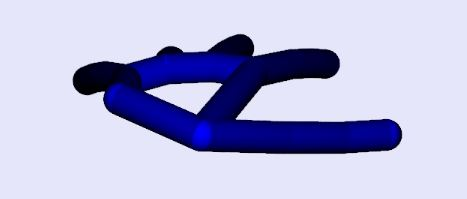
\includegraphics[scale=0.45]{Figures/4_handFlat.JPG}
\caption[Hand in Flat Orientation]{This shows the user's hand in a flat orientation; as determined by the Leap Motion sensor.}
\label{fig:handFlat}
\end{figure}
It should noted how difficult it is to see the fingers and thumb. They are only barely visible. Therefore the user would be forced to force his or her hand into a vertical position by straining their wrist just so they can see the gesture they are performing on the screen. Figures \ref{fig:handYaw} and \ref{fig:handRoll} show other orientation the hand can take; these figures show the hand after a yaw rotation and after a roll rotation respectively. Again, note the slight difficulty in figuring out the thumb and fingers positions and orientations when the hand is rolled around the z-axis. The hand that is shown in the yaw rotation in Figure \ref{fig:handYaw} is able to seen a little clearly because the wrist was strained upwards. 
\begin{figure}[H]
    \centering
    \begin{minipage}{0.5\textwidth}
        \centering
        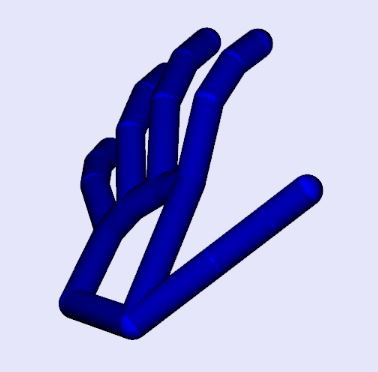
\includegraphics[scale=.55]{Figures/4_handYaw.JPG} 
        \caption[Hand with Yaw Rotation]{The user's hand after the certain yaw rotation around the y-axis.}
		\label{fig:handYaw}
    \end{minipage}\hfill
    \begin{minipage}{0.5\textwidth}
        \centering
        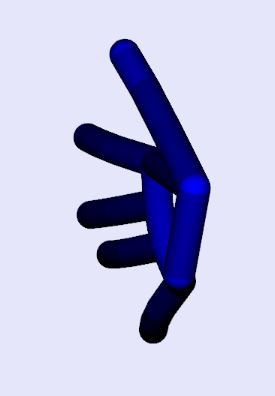
\includegraphics[scale=.55]{Figures/4_handRoll.JPG}
        \caption[Hand with Roll Rotation]{The user's hand after the certain roll rotation around the z-axis.}
        \label{fig:handRoll}
    \end{minipage}
\end{figure}
Finally all of these different orientation can of course overlap with each other to create a complex orientation of the hand as shown in Figure \ref{fig:weirdHandShake}, which shows the user's left hand in a weird handshake sort of position while being rotated to the right and tilted upwards.
\begin{figure}[H]
\centering
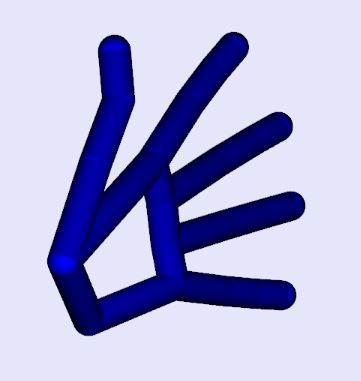
\includegraphics[scale=0.45]{Figures/4_handWeirdHandshake.JPG}
\caption[Hand in Weird Handshake Position]{This shows the user's hand in a flat orientation; as determined by the Leap Motion sensor.}
\label{fig:weirdHandShake}
\end{figure}
This chapter will explain how these different possible orientations the user's hand might be in while they are performing gestures shown on the screen are accounted for and "undone". Doing this results in the user's hand to be displayed in a set vertical orientation on the screen despite the different ways the user may have oriented their hand above the device in reality. The final resulting hand for all of the figures seen previously  will be as is shown in Figure \ref{fig:handFinalResult} after the composite rotation have transformed it to a vertical position. 
\begin{figure}[H]
\centering
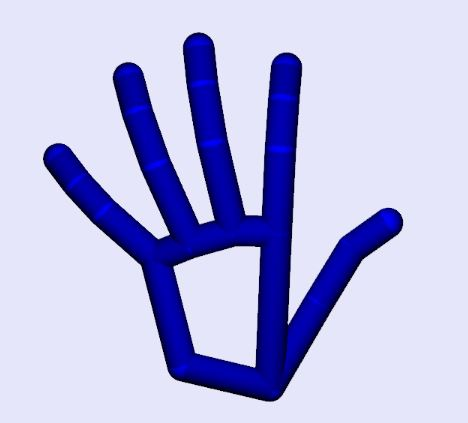
\includegraphics[scale=0.45]{Figures/4_handFinalFix.JPG}
\caption[Hand Fixed to Vertical Orientation]{This shows what the user's hand will look like after all of the possible rotational transforms have been undone and the hand has been fixed to a vertical orientation.}
\label{fig:weirdHandShake}
\end{figure}
This feature of the application makes it easier for the user to see what his or her hand is doing without requiring them to always contain their hand in a specific orientation. The goal of this application is to measure the accuracy with which a user is able to complete certain gestures, not the orientation of their hand. In fact, the algorithms that are used to grade the correctness of the user's attempted gesture do not take the user's hand orientation into account. They focus on the fingers bones and their relative orientations to each other. At the beginning of this project, one of the ideas discussed was to build some sort of rig which would be used to place the user's hand in a set orientation. However because of what will be explained in this chapter such a rig is no longer necessary.



%------------------------------------------------
%	SECTION 1 JavaFx CS vs Leap Motion CS
%------------------------------------------------
\section{JavaFx Coordinate System vs Leap Motion Coordinate System}
The Leap Motion controller has a different coordinate system from JavaFX. This distinction is very important to get out of the way as the rest of the chapter will rely on such an understanding. The coordinate system for the Leap Motion device is shown in Figure \ref{fig:leapcs}. Note the placement of the green LED light in the Leap Motion device as shows the orientation of the otherwise symmetrical picture.
\begin{figure}[H]
\centering
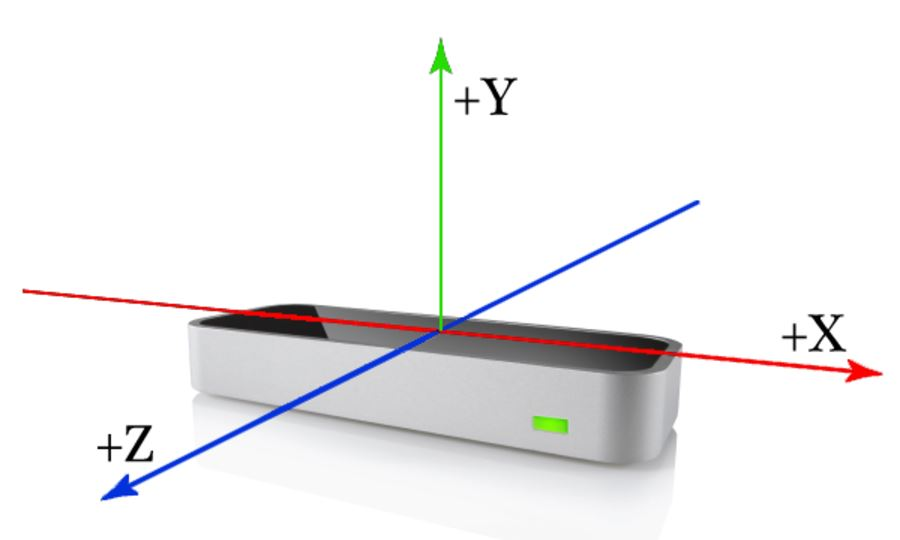
\includegraphics[scale=0.35]{Figures/4_leapCS.JPG}
\caption[Leap Motion Coordinate System]{The coordinate system that is used by the Leap Motion sensor. Data collected will based upon these axes.}
\label{fig:leapcs}
\end{figure}

This coordinate system is referred to as a right-handed coordinate system because of the easy way in which it can be represented by the first three fingers of the right hand as shown in Figure \ref{fig:lhcsRhcs}. 
\begin{figure}[H]
\centering
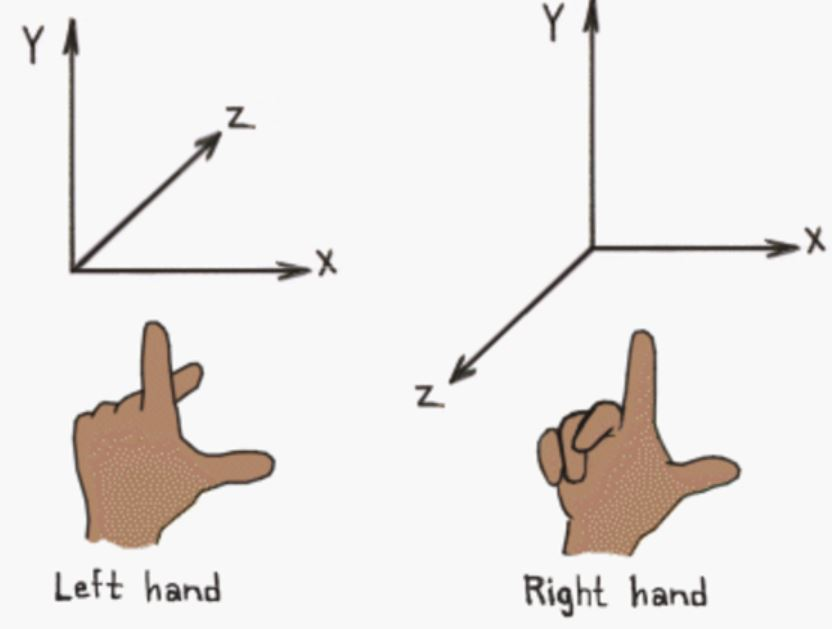
\includegraphics[scale=0.35]{Figures/4_lhrhCS.JPG}
\caption[Left vs Right Hand Coordinate System]{Left and right handed coordinate systems and how they can be shown via fingers.}
\label{fig:lhcsRhcs}
\end{figure}

In contrast, the traditional coordinate system which is used in computer science and which is what JavaFX also follows is shown in Figure \ref{fig:javafxcs}. The JavaFx coordinate system is not left handed or right handed as far as we can tell from the Figures shown. 
\begin{figure}[H]
\centering
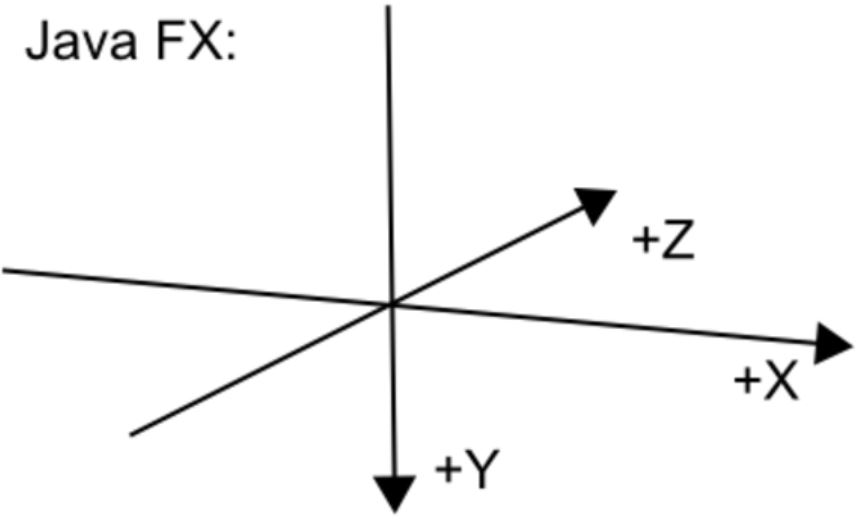
\includegraphics[scale=0.35]{Figures/4_javafxCS.JPG}
\caption[JavaFX Coordinate System]{The coordinate system used in JavaFX. Setting transforms on objects will be based on this coordinate system.}
\label{fig:javafxcs}
\end{figure}

Understanding these somewhat subtle difference and being able to switch from one context to the other was very important when considering the various rotational transforms that needed to be applied to the Hand UI model in order to straighten it to a vertical position. For example, one of the things that caused me some headaches sometimes when I was fixing and debugging my code was the fact that 3D rotations are measured in a very specific way. When it is said that some object is rotated around the y-axis by 90 degrees, this means that the if we imagine ourselves to be an observer standing on the y-axis and looking down the negative direction of this y-axis, then we would observe the object to rotate counter-clockwise about the y-axis. Therefore, it becomes very clear why it is significant to have clear understanding of the coordinate system that is being used for a particular section of code. Leap Motion data is returned with the default settings of the Leap Motion coordinate system. This data must be appropriately modified when the code using it is based upon the JavaFX coordinate system. Likewise composite rotations around certain axis might become jumbled up if one is not careful.  	


%------------------------------------------------
%	SECTION 2 Unexpected Leap Motion API Results 
%------------------------------------------------
\section{Unexpected Leap Motion API Results} 
In the course of working on this feature, which was explained in first section of this chapter, I realized that I was being returned results from the Leap Motion API that I was not expecting. I tested and debugged further into these issues until I realized some interesting things about the Leap Motion API which helped me to implement the vertical rotation of the user's hand successfully. In this section, I will go over some of the unexpected results that I obtained when I was learning more about the Leap Motion API's. I created a special Java class to help me in this endeavor which contains code samples with some simple yet illustrative scenarios which show how the Leap Motion API works.

I first noticed these problems when I was working user hand data, however, I soon realized these issues were more so with how the Vector is defined in the Leap Motion API. Therefore, the examples shown in this section will primarily be using vectors to illustrate the issues encountered, but of course these issues then extend to the collected hand data because of the nature of how Hand objects are defined in Leap Motion.


%----------------------------------- Pitch, Roll, Yaw in Leap API
\subsection{Pitch, Roll, Yaw in Leap API}
Leap Motion's Java API includes a Vector class that contains several useful operations one might need to perform. For example, it include three functions that return the pitch, roll and yaw angles for the vector. However, right away we need to understand that these angles which are returned are with respect to certain axes. The pitch() is an instance method for a vector object that will return the angle between this vector's projection onto the y-z plane and the negative z-axis. Figure \ref{fig:pitchPic} shows this. Yaw is defined to be the angle between the negative z-axis and the projection of the vector onto the x-z plane (Figure \ref{fig:yawPic}. 
\begin{figure}[H]
    \centering
    \begin{minipage}{0.5\textwidth}
        \centering
        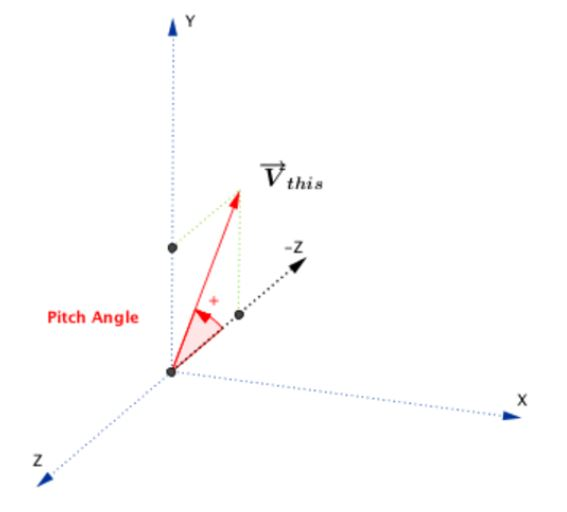
\includegraphics[scale=.55]{Figures/4_pitchPic.JPG} 
        \caption[Pitch]{Pitch angle.}
		\label{fig:pitchPic}
    \end{minipage}\hfill
    \begin{minipage}{0.5\textwidth}
        \centering
        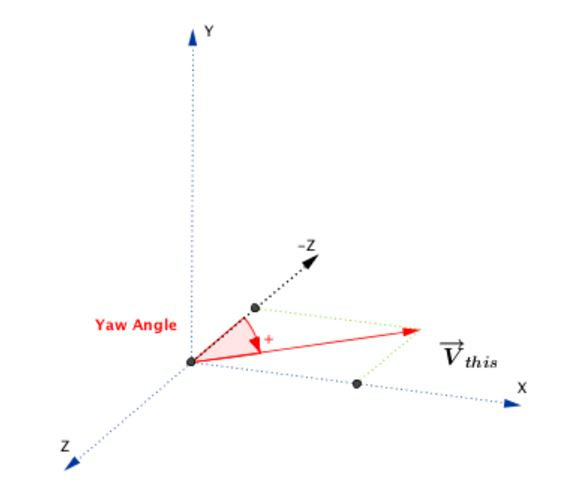
\includegraphics[scale=.55]{Figures/4_yawPic.JPG}
        \caption[Yaw]{Yaw angle.}
        \label{fig:yawPic}
    \end{minipage}
\end{figure}

roll() function is defined to be gotten by projecting the vector in question onto the x-y plane and taking the angle between this projection and the positive y-axis (which as we know is defined to be pointing upwards in the Leap Motion coordinate system and downwards in JavaFX). See Figure \ref{fig:rollPic} to get a visual understanding of how the roll angle is defined for a given vector.
\begin{figure}[H]
\centering
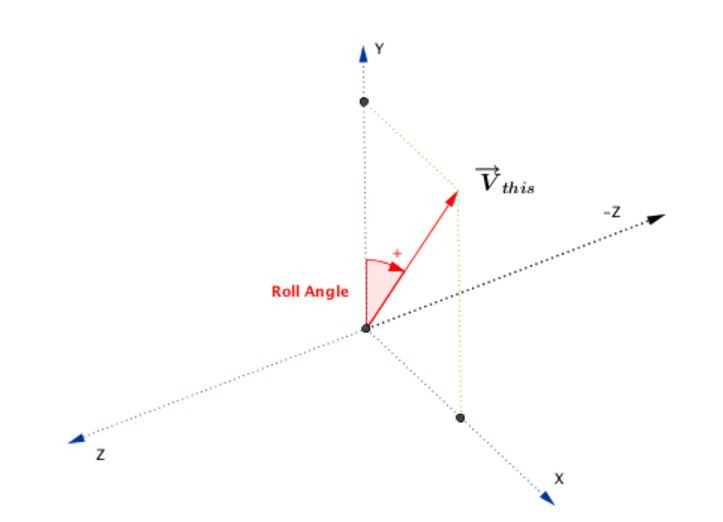
\includegraphics[scale=0.35]{Figures/4_rollPic.JPG}
\caption[Roll]{Roll angle as defined in Leap Motion documentation.}
\label{fig:rollPic}
\end{figure}



%----------------------------------- Negative Zeros and Flipped Axes
\subsection{Negative Zeros and Flipped Axes}
During my testing, I realized that the Vector class returns some strange results when we test the pitch() function with the simple x-axis unit vector <1,0,0>. One would expect that the pitch would be zero, since the projection of the x-axis unit vector onto the y-z plane is zero. However, as the debugging result in Figure \ref{fig:negZero} shows, that was not the case. 
\begin{figure}[H]
\centering
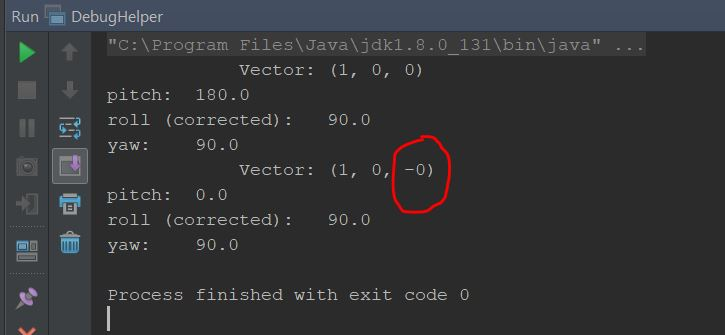
\includegraphics[scale=0.35]{Figures/4_negZero.JPG}
\caption[Pitch() Debugging]{A simple example's run output that demonstrates the negative zeros and their importance in Leap Motion API.}
\label{fig:negZero}
\end{figure}

It appears to be that a negative zero must be supplied in the z-component of the vector to get a zero pitch angle. When I found this out, I was very surprised as it was the first time I realized that there was such a thing as a negative floating point zero. However,  another thing to note is that in the debug output, I have the word "corrected" next to the roll angle. 

Like the pitch() angle, I noticed something that was a bit strange about the results the roll() function was returning during my debugging. It was returning 135 degrees when I was expecting it to return 45 degrees (see Figure \ref{fig:uncorrectedRoll}) because the vector it is being tested on makes such a projection onto the x-y plane that the roll should be 45. I think the documentation page either has a mistake the roll() method or maybe the Vector class has a error in the way the roll method is defined. 
\begin{figure}[H]
\centering
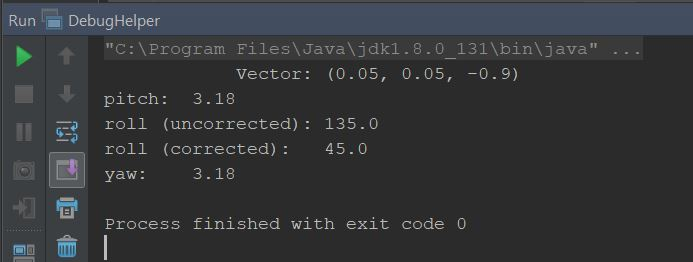
\includegraphics[scale=0.35]{Figures/4_rollUncorrected.JPG}
\caption[Roll Debugging]{The roll() angle returned for a vector needs to be "corrected".}
\label{fig:uncorrectedRoll}
\end{figure}

The angle being returned is actually between the negative y-axis (Leap Motion coordinate system) and the projection. Therefore I wrote my own correctedRoll() which basically takes a given roll angle and subtracts it from 180 degrees to return a roll angle that is in accordance to how roll() is defined in Leap Motion documentation. In response to finding out about these problems, I wrote my own methods to find pitch, roll and yaw when I was dealing with hand objects. The code for one of these methods is shown in Figure \ref{fig:pitchCode}.
\begin{figure}[H]
\centering
\begin{lstlisting}
private float getPitch(Hand h) {
	//angle of hand direction to y-axis
	float angleAmount = (float) Math.toDegrees(h.direction().angleTo(Vector.yAxis()));
	//switch direction of angle
	if (h.direction().getZ() > 0.0f) {
		return (-1.0f * angleAmount); //returning a -negative angle to "undo" the positive pitch noticed in hand
	} else {
		//99 % of the time, pitch will be a positive angle, so this case will run most of the time.
		return angleAmount;
	}
}
\end{lstlisting}
\caption[getPitch() Function]{This function returns the pitch of the hand object as the angle the hand makes to the x-z plane.}
\label{fig:pitchCode}
\end{figure}
This method does not rely on projections to the y-z plane to find out the pitch of the hand. Intuitively, when I imagined the pitch of the hand model to be to angle it is making to the x-z plane; regardless of which direction the wrist or the fingers of the hand are pointing in. The Leap pitch() function expects the direction of the hand to be relatively inline with the z-axis in order to give a valid pitch measurement. The method I defined does not have this restriction and is able to return an informative pitch angle no matter if the user has rotated his/hand around the y-axis. I calculate the yaw for a particular hand in the same fashion, except for that function I take the angle between the direction of the hand and the negative z-axis. 


%------------------------------------------------
%	SECTION 3 Simplified Hand Model
%------------------------------------------------
\section{Simplified Hand Model}
	
	
%------------------------------------------------
%	SECTION 4 Composite Linear Transformations
%------------------------------------------------
\section{Composite Linear Transformations}
--combine these two. 
%------------------------------------------------
%	SECTION 5 Rotational Matrix
%------------------------------------------------
\section{Rotational Matrix}






\chapter{Scoring of Gestures}

\label{Chapter5_scoring} 

\begin{comment}
-------------------------------------------------
%								Chapter layout
5. Scoring of Gestures
	a. Angle Based Comparison Function
	b. Component Based Comparison Function
-------------------------------------------------
\end{comment}

%------------------------------------------------
%	SECTION 1 Angle Based Comparison Function
%------------------------------------------------
\section{Angle Based Comparison Function}
%description of algorithm and introduction to compare() function
This is the first way by which a hand gesture is scored. This scoring method compares one hand against another; namely, it is usually comparing the user's hand versus the target hand shown on the screen that the user was trying to imitate. It uses the angles between the three foremost bones, (distal, intermediate, proximal), of the five fingers as the primary means of determining how close a user's hand is to the target hand. It also uses the angle the wrist makes to the arm in its calculations to determine the final score for the hand. Figure \ref{fig:compare1} shows some important parts of the compare() function which scores the angular similarities between two hands. This function first makes sure that the two hands that are being compared are of the same kind; ie the hands must both be left or both must be right, otherwise the result of the compare() function will be 0. It then finds angles between adjacent finger bones in both hands and compares the two angles for the amount of similarity between them. This similarity between the two angles, which is the result of the compareAngles() method call, will be a number between 0 and 1. A weight applied to this similarity measure and then the result added to the summation variable x. This function relies on some weight parameters, see Figure \ref{fig:weights}, that are set higher for the longer bones that are closer to the knuckles. For example the proximal bones have a weight of 4; the intermediate bones have a weight of 2 and the distal bones have a weight of 1. This is because the bigger bones closer to the palm of the hand are a bit more limited in their mobility. Therefore, determining correlation between these corresponding bigger bones such as proximal has a higher influence on the overall value of the compare() function. 
\begin{figure}[H]
\centering
\begin{lstlisting}
public double compare(Hand h1, Hand h2) {
	//check if both hands are of the same type.
	if (h1.isLeft() == h2.isLeft()) {
		double x = 0;
		//wrist
		x += compareAngles(angleWristArm(h1), angleWristArm(h2))* weight_wrist;
		//five fingers "proximal". compareAngles always returns between 0-1
		x += compareAngles(anglePinkyProximal(h1), anglePinkyProximal(h2))*weight_pinky_proximal;
		x += compareAngles(angleRingProximal(h1), angleRingProximal(h2))* weight_ring_proximal;
		x += compareAngles(angleMiddleProximal(h1), angleMiddleProximal(h2))* weight_middle_proximal;
		x += compareAngles(angleIndexProximal(h1), angleIndexProximal(h2))* weight_index_proximal;
		x += compareAngles(angleThumbProximal(h1), angleThumbProximal(h2))* weight_thumb_proximal;
		//five fingers "intermediate"
		x += compareAngles(anglePinkyIntermediate(h1), anglePinkyIntermediate(h2))* weight_pinky_intermediate;
		...
		//five fingers "distal"
		x += compareAngles(anglePinkyDistal(h1), anglePinkyDistal(h2))* weight_pinky_distal;
		...
		x /= totalWeight();
		return x;
	} else{
		//if comparing left hand to right hand (or vice versa), return 0
		return 0; 
	}
}
\end{lstlisting}
\caption[Angular Comparison Function]{This snippet of code shows the main skeleton of the function that determines the similarity between two hands by comparing angles between various bones in the hands.}
\label{fig:compare1}
\end{figure}


\begin{figure}[H]
\centering
\begin{lstlisting}
//weights for various bone types 
static double weight_pinky_proximal = 4;
static double weight_pinky_intermediate = 2;
static double weight_pinky_distal = 1;
...
\end{lstlisting}
\caption[Bone Weights in Angular Comparison Function]{An example of the weights set for different bone types in the pinky finger.}
\label{fig:weights}
\end{figure}


%compareAngles() function
It is also worth looking into how the compareAngles() function is defined as this function determines what percentage of the weights get applied. It takes in two angles as it parameters. These angles are determined via various functions which find angles between consecutive bones of a specific finger. An example of one such function is shown in Figure \ref{fig:angleIndexDistal} which shows how the angle between the distal bone and the intermediate bone in the index finger is determined. The angle returned by these functions will always be less than 180 degrees because of the way the angleTo() function is defined in the Leap Motion API. 
\begin{figure}[H]
\centering
\begin{lstlisting}
private float angleIndexDistal(Hand h) {
	Vector direction1 = h.fingers().get(1).bone(Bone.Type.TYPE_DISTAL).direction();
	Vector direction2 = h.fingers().get(1).bone(Bone.Type.TYPE_INTERMEDIATE).direction();
	float rawAngle = direction1.angleTo(direction2);//always less than 180
	return normalize(rawAngle, h);//flips angle on xAxis if palm facing upwards
}
\end{lstlisting}
\caption[angleIndexDistal() Function]{This function is one example of how the angles between adjacent bones are determined.}
\label{fig:angleIndexDistal}
\end{figure}

The compareAngles() is a mathematical function that determines the similarity between two angles passed into it by using the cosine trigonometry function. It will return an number between 0 and 1. It first finds the difference between the two angels. If the angles are so far apart and the distance is greater than 45 degrees, then the function will return a zero to indicate that there is not any meaningful closeness between the two angles being compared. Figure \ref{fig:compareAngles} shows this function's code. 
\begin{figure}[H]
\centering
\begin{lstlisting}
private double compareAngles(float angle1, float angle2) {
	double differenceBtwAngles = Math.abs(angle1-angle2);
	//tmp can be at most pi/4 = 45
	double tmp = Math.min(differenceBtwAngles, Math.PI/4);
	//if tmp is exactly 45, will return 0. cos(90) = 0.
	return Math.cos(2*tmp);
}
\end{lstlisting}
\caption[compareAngles() Function]{This function determines how similar (or close together) two angles using cosine.}
\label{fig:compareAngles}
\end{figure}



	


%------------------------------------------------
%	SECTION 2 Component Based Comparison Function
%------------------------------------------------
\section{Component Based Comparison Function}
The second way by which a score is assigned to a hand representing an attempted gesture will be discussed in this section. 

%descripton of algorithm
The idea behind this method is to take a given hand and decompose it into smaller component that can be scored individually. Then these components scores will be combined to arrive at the cumulative score for the entire hand. Each finger is seen as a component. After considering all of the gestures being tested in this project, I realized that each finger can be in one of three main kinds of poses. All of the fingers except for the thumb are only seen in some variations of being straight, or being curved. The thumb, however, has its own special kind of pose, which deals with connecting to other fingers. For example in some of the gestures the thumb is touching the pinky; in some gestures it is touching the middle finger. Therefore, the third possible pose is represented by a finger name, such as "pinky" or "index" etc., and it represents the finger the thumb is touching in the gesture being analyzed. The way the algorithm is designed, it makes sense to assign this dynamic third pose to the thumb only. Figure \ref{fig:gestureComponents1} and Figure \ref{fig:gestureComponents2} shows one of the gestures used in this project, namely gesture9Left, to illustrate what is meant by the different poses different components of the hand can take. As we can see, all of the fingers are straight; the ring finger is curved; and the thumb is touching the ring finger. This "pose signature" of this gesture as it is used in code is shown in Figure \ref{fig:gesture9PoseSignature}. The pose signature for a certain gesture is the same regardless of whether left or right hand is being used. That is why the code sample shows two case statements for gesture9Left and gesture9Right. 

\begin{figure}[H]
    \centering
    \begin{minipage}{0.45\textwidth}
        \centering
        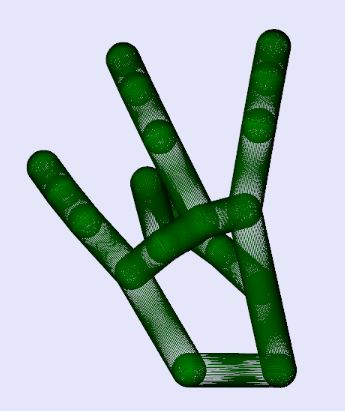
\includegraphics[scale=.5]{Figures/straight_curved_thumb1.JPG} % first figure itself
        \caption{Gesture showing different finger poses.}
		\label{fig:gestureComponents1}
    \end{minipage}\hfill
    \begin{minipage}{0.45\textwidth}
        \centering
        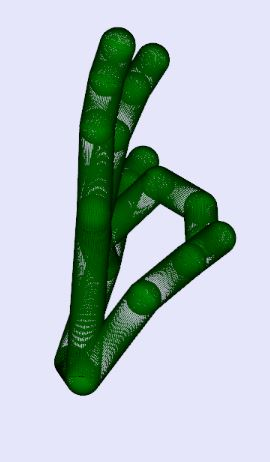
\includegraphics[scale=.5]{Figures/straight_curved_thumb2.JPG} % second figure itself
        \caption{Same gesture after a 90 degree rotation.}
        \label{fig:gestureComponents2}
    \end{minipage}
\end{figure}


\begin{figure}[H]
\centering
\begin{lstlisting}
case "gesture9Left":
case "gesture9Right":
	fingerPoseMap.put("index", "straight");
	fingerPoseMap.put("middle", "straight");
	fingerPoseMap.put("ring", "curved");
	fingerPoseMap.put("pinky", "straight");
	fingerPoseMap.put("thumb", "ring");
	break;
\end{lstlisting}
\caption[Finger Pose Mapping]{In the component based scroing, each gesture type gets a certain mapping for the kinds of poses fingers are expected to be in for that gesture.}
\label{fig:gesture9PoseSignature}
\end{figure}


% compare function and its helper functions
The comparison function for the component based scoring of hand gestures is shown in Figure \ref{fig:compare2}. It returns a number 0-100 just like the angle based comparison function to indicate the score for the hand being graded. This function gets the fingers for the hand and goes through and finds the individual grades for each finger. Then it combines the into a cumulative grade by weighing the fingers equally. 
\begin{figure}[H]
\centering
\begin{lstlisting}
public static int compare(Hand h, String gestureType) {
	FingerList fingerList = h.fingers();
	//make sure you have five fingers
	if (fingerList.count() == 5) {
		//calculate grades for each finger
		HashMap<String, Double> grades = getFingersGradedMap(getFingerHashMap(fingerList), getFingerPoseMap(gestureType));
		//grade for whole hand
		double totalGrade = cumulativeGrade(grades);
		//score 0-100
		return (int) (totalGrade * 100.0);
	}
	return -1;
}
\end{lstlisting}
\caption[Component Based Comparison Function]{}
\label{fig:compare2}
\end{figure}

To give a clearer idea about how the fingers actually get graded, the gradeFinger() function is shown in Figure \ref{fig:gradeFinger}. This function relies on three helper functions which calculate the straightness and curvedness of fingers and a function which returns the score for the thumb. 
\begin{figure}[H]
\centering
\begin{lstlisting}
private static double gradeFinger(HashMap<String, Finger> fingerMap, Finger f, String pose) {
	if (pose.equals("straight")) {
		return straightnessOfFinger(f);
	} else if (pose.equals("curved")) {
		return curvednessOfFinger(f);
	}
	//thumb is not touching any finger
	else if (pose.equals("thumb")) {
		return straightnessOfFinger(f);
	}
	//thumb touching other fingers
	else {
		Finger theFingerThumbTouches = fingerMap.get(pose);
		return getThumbScore(f, theFingerThumbTouches);
	}
}
\end{lstlisting}
\caption[gradeFinger() Function]{Given a finger a certain pose, this function returns a grade (0-1) for that finger. It uses helper functions to calculate grades for a finger in one the three main kinds of poses.}
\label{fig:gradeFinger}
\end{figure}		

Two of these helper functions, the straightnessOfFinger() and curvednessOfFinger() are shown in Figure \ref{fig:straightCurvedHelperFunctions}. These functions first find the sum of the angle between consecutive bones in the finger that is being graded. For a perfectly straight finger, the sum of these angles should be around 0 degrees. However, to allow for some leniency in the grading 30 degrees are subtracted from the sum of the angles. This allows for a buffer for the user that we intuitively as humans might guage as being relatively straight. For measuring the curvedness of a finger, the sum of the angles between the bones of the fingers should be as close to 270 as possible. However, again a buffer was provided to allow for not perfectly curled fingers to still be valid enough to return a good score.Of course these parameters can be adjusted if this application was used in the real world. These were what I felt were good parameters when I wrote these grading functions.
\begin{figure}[H]
\centering
\begin{lstlisting}
private static double straightnessOfFinger(Finger f) {
	//best case = 0; worst case is: 90+90+90 = 270.
	double sumOfAngles = getSumOfThreeAnglesBetweenFingerBones(f);
	sumOfAngles = sumOfAngles - 30;//offset by 30 degrees
	double score = sumOfAngles / 270;//closer to 0 means a better score
	score = 1 - score;//conventional scale: 0 = bad, 1 = good.
	return snapScore0to1(score);
}
private static double curvednessOfFinger(Finger f) {
	//best case is: 90+90+90 = 270; adjusted bestcase = 210; worst case = 0;
	double sumOfAngles = getSumOfThreeAnglesBetweenFingerBones(f);
	double score = sumOfAngles / 210;//closer to 1 means a better score
	return snapScore0to1(score);
}
\end{lstlisting}
\caption[straightnessOfFinger() and curvednessOfFinger()]{These helper functions are similar to each other. They are used in grading the four fingers.}
\label{fig:straightCurvedHelperFunctions}
\end{figure}		

The helper function getThumbScore(), shown in Figure \ref{fig:getThumbScore} is the more complicated of the three. The way a score is calculated for a thumb is by finding the distance between the tip bone of the thumb and any of the three outermost bones on the finger the thumb is supposed to be touching. The smallest distance is chosen as the tip of the thumb might be closer to any three of the distal, intermediate or proximal bones. This is because some people rest their thumb on the tip of the distal bone, others rest on top of the distal or the intermediate. This distance is scaled down by the smallest bone length multiplied by a scaling factor. Like the other two functions, straightnessOfFinger() and curvednessOfFinger(), the score that is returned is snapped to be between 0-1. 
\begin{figure}[H]
\centering
\begin{lstlisting}
private static double getThumbScore(Finger thumb, Finger otherFinger) {
	//bones in thumb and finger
	HashMap<String, Bone> thumbMap = getHashMapOfBonesFromFinger(thumb);
	HashMap<String, Bone> fingerMap = getHashMapOfBonesFromFinger(otherFinger);
	//get center point of thumb's tip bone
	Vector thumbTip = thumbMap.get("distal").center();
	//finger bones
	Bone d = fingerMap.get("distal");
	Bone i = fingerMap.get("intermediate");
	Bone p = fingerMap.get("proximal");
	//length of bones
	float smallestBoneLength = (Math.min(Math.min(d.length(), i.length()), p.length()));
	//distances from thumb tip to finger bones
	float d1 = thumbTip.distanceTo(d.center());
	float d2 = thumbTip.distanceTo(i.center());
	float d3 = thumbTip.distanceTo(p.center());
	double minDistance = (double) (Math.min(Math.min(d1, d2), d3));
	//scale and score
	double distanceScaledByBoneLength = minDistance / (smallestBoneLength * 3);
	double score = 1 - distanceScaledByBoneLength;
	return snapScore0to1(score);
}
\end{lstlisting}
\caption[getThumbScore() Helper Function]{This function calculates the grade for the thumb that is supposed to be touching one of the four fingers. It calculates this score by distances rather than using angles.}
\label{fig:getThumbScore}
\end{figure}

%doenst need a target hand to compare against. explain why this is good. 
One final thing to note about this comparison function is that it does not rely on a target hand for the comparison. Instead it relies on set gesture poses that are expected for the different gestures to arrive at its score. Therefore, it is more stable form of comparison. If the target hands are themselves not very good examples of the gestures being displayed, the angle based comparison method's performance could be unnecessarily affected. 
 
\chapter{Application User Interface }

\label{Chapter6_appUI} 

\begin{comment}
-------------------------------------------------
%								Chapter layout
6. Application User Interface 
	a. Main Layout
	b. User Specific Data Collection
	c. Visual Rotation of Gesture
	d. Tabular Display of Data
	e. Writing and Reading from CSV
	f. Artifacts and Distribution
		i. Leap App Store
		ii. IDE Build Process and Batch Script
-------------------------------------------------
figures needed:
homescreen,

load/create new user screen. 
load/create new user screen. (with dropdown showing)

X->testing screen. also showing user hand. 
X->testing screen after rotation done. also showing user hand. 

analyze screen.
load folder button clicked. opened dialog. 
save to csv opened dialog. 
\end{comment}


In this chapter some of the useful UI features of the application will be discussed. 

%------------------------------------------------
%	SECTION 0 Main Layout
%------------------------------------------------
\section{Main Layout}

The application has three main scenes. One is the home screen which shows buttons to take the user to the other two scenes. It also contains two radio buttons to allow the user to select which hand (left or right) he/she will be testing with the gestures. Figure  \ref{fig:homescreen} shows the layout of the home screen. 

\begin{figure}[H]
\centering
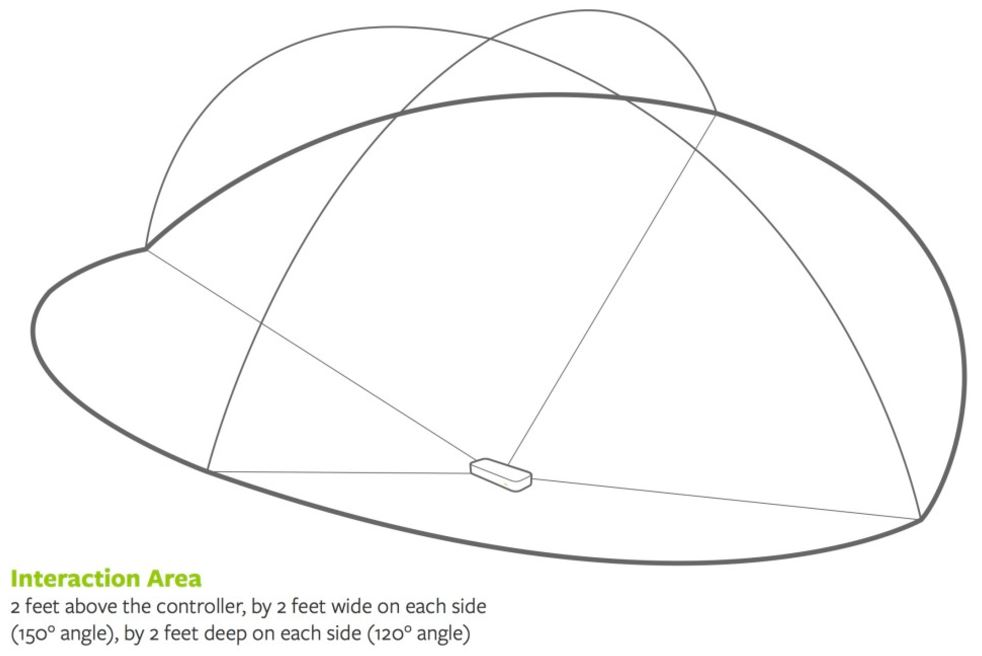
\includegraphics[scale=0.35]{Figures/LeapInteractionArea.JPG}
\caption[Home Screen Layout]{The scene that the user sees intially when they load the application.}
\label{fig:homeScreen}
\end{figure}

The user can click on the Analyze Data button to got 


talk about three scenes and show pics. show what happens where and 
what the typical user would do. 
take data and analyze it for problems. 
and then go fix those problems. 
also save data to csv. read from csv. 
say some things will be dicussed in other sections. 


%------------------------------------------------
%	SECTION 1 User Specific Data Collection
%------------------------------------------------
\section{User Specific Data Collection}


show the 2 figures. explain why you needed ot make users. meeting with clinicians. working product demonstration. agile. as opposed ot waterfall (this should go in conclusion). 

 

%------------------------------------------------
%	SECTION 2 Visual Rotation of Gesture
%------------------------------------------------
\section{Visual Rotation of Gesture}

same as above. 

%------------------------------------------------
%	SECTION 3 Tabular Display of Data
%------------------------------------------------
\section{Tabular Display of Data}

editable picture. show code. 
%------------------------------------------------
%	SECTION 4 Writing and Reading from CSV
%------------------------------------------------
\section{Writing and Reading from CSV}


%------------------------------------------------
%	SECTION 5 Artifacts and Distribution
%------------------------------------------------
\section{Artifacts and Distribution}

%----------------------------------- Leap App Store
\subsection{Leap App Store}

%----------------------------------- IDE Build Process and Batch Script
\subsection{IDE Build Process and Batch Script}



\chapter{Data Collection}

\label{Chapter7_dataCollection} 

\begin{comment}
-------------------------------------------------
%								Chapter layout
7. Data Collection
	a. The Approach Taken
	b. User Feedback
-------------------------------------------------
\end{comment}

Data collection for this project happened in two main ways. One was via the clinicians, who represented the clients who would be using the software this project was building on patients in John Radcliffe Hospital. The other way was through myself reaching out to students and other people around my college to ask them if they would like to participate in the data collection part of my MSc project.  


%------------------------------------------------
%	SECTION 1 The Approach Taken
%------------------------------------------------
\section{The Approach Taken}
Throughtout the course of this entire project, I met with the clinicians, Dr Samrah Ahmed, Dr Christopher Butler, and Nikolas Drummond, several times to discuss the application as it was being designed and built. The featues they requested were fully tried to be implemented in this software and in the final visit to the hospital, the final version of the application was delivered for the clinicians for testing and collecting some control data. They feedback received from them was very positive and all of their major UI enhancements and usability features were implemented satisfactorily. 

%talk about how you went about collecting data from users around college. how you approached them. how you explained your project to them and demoed them. how you had to be patient. and guide them. how you bought chocolate to encourage them and mention the short survey you had them complete. how long it took. 

%talk about how hard it is. you have to go out and buy chocolate. you have to search for people. you have to approach them when they are busy. you are embarassed to disturb them. it is a busy time of the year. but you have to overcome that fear and reach out and collect your data. you make new friends. you gain a new found confidence. <-- talk about this. reference requirements engineering if you want or need to. 



%------------------------------------------------
%	SECTION 2 User Feedback
%------------------------------------------------
\section{User Feedback}




\chapter{Results and Analysis}

\label{Chapter8_results} 

\begin{comment}
-------------------------------------------------
%								Chapter layout
8. Results and Analysis
-------------------------------------------------
\end{comment}

this is the results chapter. 

\chapter{Conclusion}

\label{Chapter9_conclusion} 

\begin{comment}
-------------------------------------------------
%								Chapter layout
9. Conclusion
	a. Future Work
		i. Scoring Functions Improvement
		ii. Other Improvements (UI, distribution, change of framework. electron ui -> web based. )
	b. Personal Note
-------------------------------------------------
\end{comment}

This is the conclusion ...

%------------------------------------------------
%	SECTION 1 Future Work
%------------------------------------------------
\section{Future Work}
\begin{comment}
% should talk about how it can be made better. maybe can weigh different fingers differently. maybe in certain gestures a certain finger is more imprortant.

	-angle, dont die if left/right. 
	-need to have a way of returning 0 if one of the fingers is compeletley off. 
	-need to be able to parameterize by finger level. (compare2). if in gesture10 we expect the pinky to be a little curved, should be able to set that parameter on that pinky in that gesture. rather than entire algorithm. need more fine tune parameterization. 
	
	
	
show the 2 figures about loading/creating user. explain why you needed ot make users. meeting with clinicians. working product demonstration. agile. as opposed ot waterfall (this should go in conclusion). 
- in the same thread, could also explain how the rotation of the hand was also the clinician's idea. 
\end{comment}




%------------------------------------------------
%	SECTION 2 Personal Note
%------------------------------------------------
\section{Personal Note}
\begin{comment}

using goals is very helpful. 
break down of tasks. 
also stopping middle of doing something fun. this will make starting again easier. this also helps a lot in writing.
--writing is a big monster.

functional programming is so much better. 

learning things on the run. stackoverflow. learning to debug.

github. branches. going back in history. 
 
latex. 









\end{comment}
\end{comment}

%----------------------------------------------------------------------------------------
%	THESIS CONTENT - APPENDICES
%----------------------------------------------------------------------------------------

\appendix % Cue to tell LaTeX that the following "chapters" are Appendices

% Include the appendices of the thesis as separate files from the Appendices folder
% Uncomment the lines as you write the Appendices
\begin{comment}
% Appendix A

\chapter{Frequently Asked Questions} % Main appendix title

\label{AppendixA} % For referencing this appendix elsewhere, use \ref{AppendixA}

\section{How do I change the colors of links?}

The color of links can be changed to your liking using:

{\small\verb!\hypersetup{urlcolor=red}!}, or

{\small\verb!\hypersetup{citecolor=green}!}, or

{\small\verb!\hypersetup{allcolor=blue}!}.

\noindent If you want to completely hide the links, you can use:

{\small\verb!\hypersetup{allcolors=.}!}, or even better: 

{\small\verb!\hypersetup{hidelinks}!}.

\noindent If you want to have obvious links in the PDF but not the printed text, use:

{\small\verb!\hypersetup{colorlinks=false}!}.

%\include{Appendices/AppendixB}
%\include{Appendices/AppendixC}
\end{comment}
%----------------------------------------------------------------------------------------
%	BIBLIOGRAPHY
%----------------------------------------------------------------------------------------

\printbibliography[heading=bibintoc]

%----------------------------------------------------------------------------------------

\end{document}  
